\chapter{$D^0 \to \mu^+\mu^-$ Branching Fraction Measurement}

\section{Analysis overview}

\label{sec:analysis_overview}

TODO: discuss blinding

\section{Triggers and datasets}

\subsection{Data samples}

\label{subsec:data_samples}

The events used for this analysis are collected from proton-proton collisions at the LHC at a center of mass of 13.6 TeV. Specifically, we use data from the CMS detector during the years 2022 and 2023. The CMS collaboration marks specific run ranges as good runs and groups them into datasets marked with letters. The data we use is denoted as 2022C, 2022D, 2022E, 2022F, 2022G, 2023C, and 2023D. 

There are two triggers used for the analysis:
\begin{enumerate}
    \item The \texttt{HLT\_DoubleMu4\_3\_LowMass} trigger is used to collect $D^{*\pm} \to D^0 \pi^\pm, D^0 \to \mu^+ \mu^-$ signal events by triggering on the dimuon final product. During the collection of the data samples of the analysis, the trigger was virtually unchanged and unprescaled, making it convenient to use for signal collection.
    \item The \texttt{HLT\_ZeroBias} trigger was used to collect $D^{*\pm} \to D^0 \pi^\pm, D^0 \to \pi^+ \pi^-$ normalization events. Unlike the signal trigger, this trigger does not filter for a specific signature. However, the expected branching fraction of $D^{*\pm} \to D^0 \pi^\pm, D^0 \to \pi^+ \pi^-$ is large enough to generate a sufficient number of desired events. During the collection of the data samples of the analysis, the trigger was virtually unchanged and was prescaled at the HLT and L1 triggers on the order of 1e6. 
\end{enumerate}

TODO: calculate exact prescaling factor $S_{ZB} = \frac{\text{total luminosity}}{\text{ZeroBias luminosity}}$

TODO: add full length of dataset tables and perform the above calculation.

The events collected by these two triggers and grouped into two datasets, ZeroBias and Parking DoubleMuonLowMass, respectively. We use the NanoAOD file format, designed by CMS to contain ntuples of per-event information and used for most analysis at CMS. Specifically, we use the NanoAODv12 recipe which is processed from MiniAOD. In this processing, we apply the muon data certification to ensure high quality muon objects. 

\subsection{Backgrounds}
\label{subsec:backgrounds}

A key component of the analysis is the accurate modeling of background, specifically because of how small the anticpated limit of the signal strength is. There are two main types of backgrounds to consider: 
\begin{enumerate}
    \item Combinatorial backgrounds: backgrounds which are characterized by noise from random combinations of particles produced in secondary particle collisions. 
    \item Peaking backgrounds: backgrounds which are characterized by a peaking structure near the signal region.
\end{enumerate}

\subsubsection{Combinatorial Backgrounds}

Combinatorial backgrounds are signals that originate from random combinations of particles that do not come from a common physical process. The existence of combinatorial backgrounds is present in virtually every experiment performed at the LHC due to the large amounts of events generated in each proton-proton bunch collision. Combinatorial backgrounds are often characterized by smooth, non-peaking shapes due to the lack of a unifying physical process to generate a peak. There are many shapes that are used to fit to combinatorial backgrounds, with the most common being exponential functions or polynomial functions. The functions allow for the needed degrees of freedom and overall shape to converge on the smooth combinatorial shape. In other applications, more specific combinatorial functions are derived to properly model the background. 

\subsubsection{Peaking Backgrounds}

Unlike combinatorial backgrounds, peaking backgrounds must be carefully studied to ensure that the background peak in the signal region is not modeled as signal. These peaking backgrounds occur most commonly from detector misreconstruction. For example, pions can be misreconstructed as muons, resulting in some $D^0 \to \pi^+ \pi^-$ events being reconstructed as $D^0 \to \mu^+ \mu^-$ events, causing a peaking background near the signal region. Specifically, we know that pions and kaons are the only 2 particles which are (1) common decay products of the $D^0$ and (2) are relatively frequently misreconstructed as muons\footnote{See section TODO: add section for pion and kaon fake rates}. Therefore, the candidates for peaking background are two body hadronic decays of the $D^0$ meson and non-$D^{*\pm} \to D^0 \pi^\pm$ decays. 

For each of the peaking backgrounds, we check their $\Delta m$ and dimuon mass against the $\Delta m$ and dimuon mass of the signal. While the non-$D^{*\pm} \to D^0 \pi^\pm$ decays exhibit a dimuon mass distribution which is virtually identical to the signal, their $\Delta m$ contribution is expected to be combinatorial so they do no overlap with the signal's signature. The dominate two body hadronic decays of the $D^0$ meson therefore are the only contributions to peaking background and are listed below.
\begin{enumerate}
    \item $D^0 \to \pi^+ \pi^-$
    \item $D^0 \to K^\pm \pi^\mp$
    \item $D^0 \to K^+ K^-$
    \item $D^0 \to \pi^\pm \mu^mp$
\end{enumerate}
For each of these, we use \texttt{TGenPhaseSpace} to simulate the effects of the misreconstructed on the peaking background distributions in both $\Delta m$ and the invariant dimuon mass and compare them to the signal distribution. As can be seen in figure \ref{fig:reconstructed_D0_comparison}, every decay except $D^0 \to \pi^+ \pi^-$ gives a distribution which is distinct from the signal distribution in either $\Delta m$ or the dimuon invariant mass. Therefore, the only peaking distribution which we must model and account for is $D^0 \to \pi^+ \pi^-$. 

\begin{figure}[htp]
    \begin{center}
      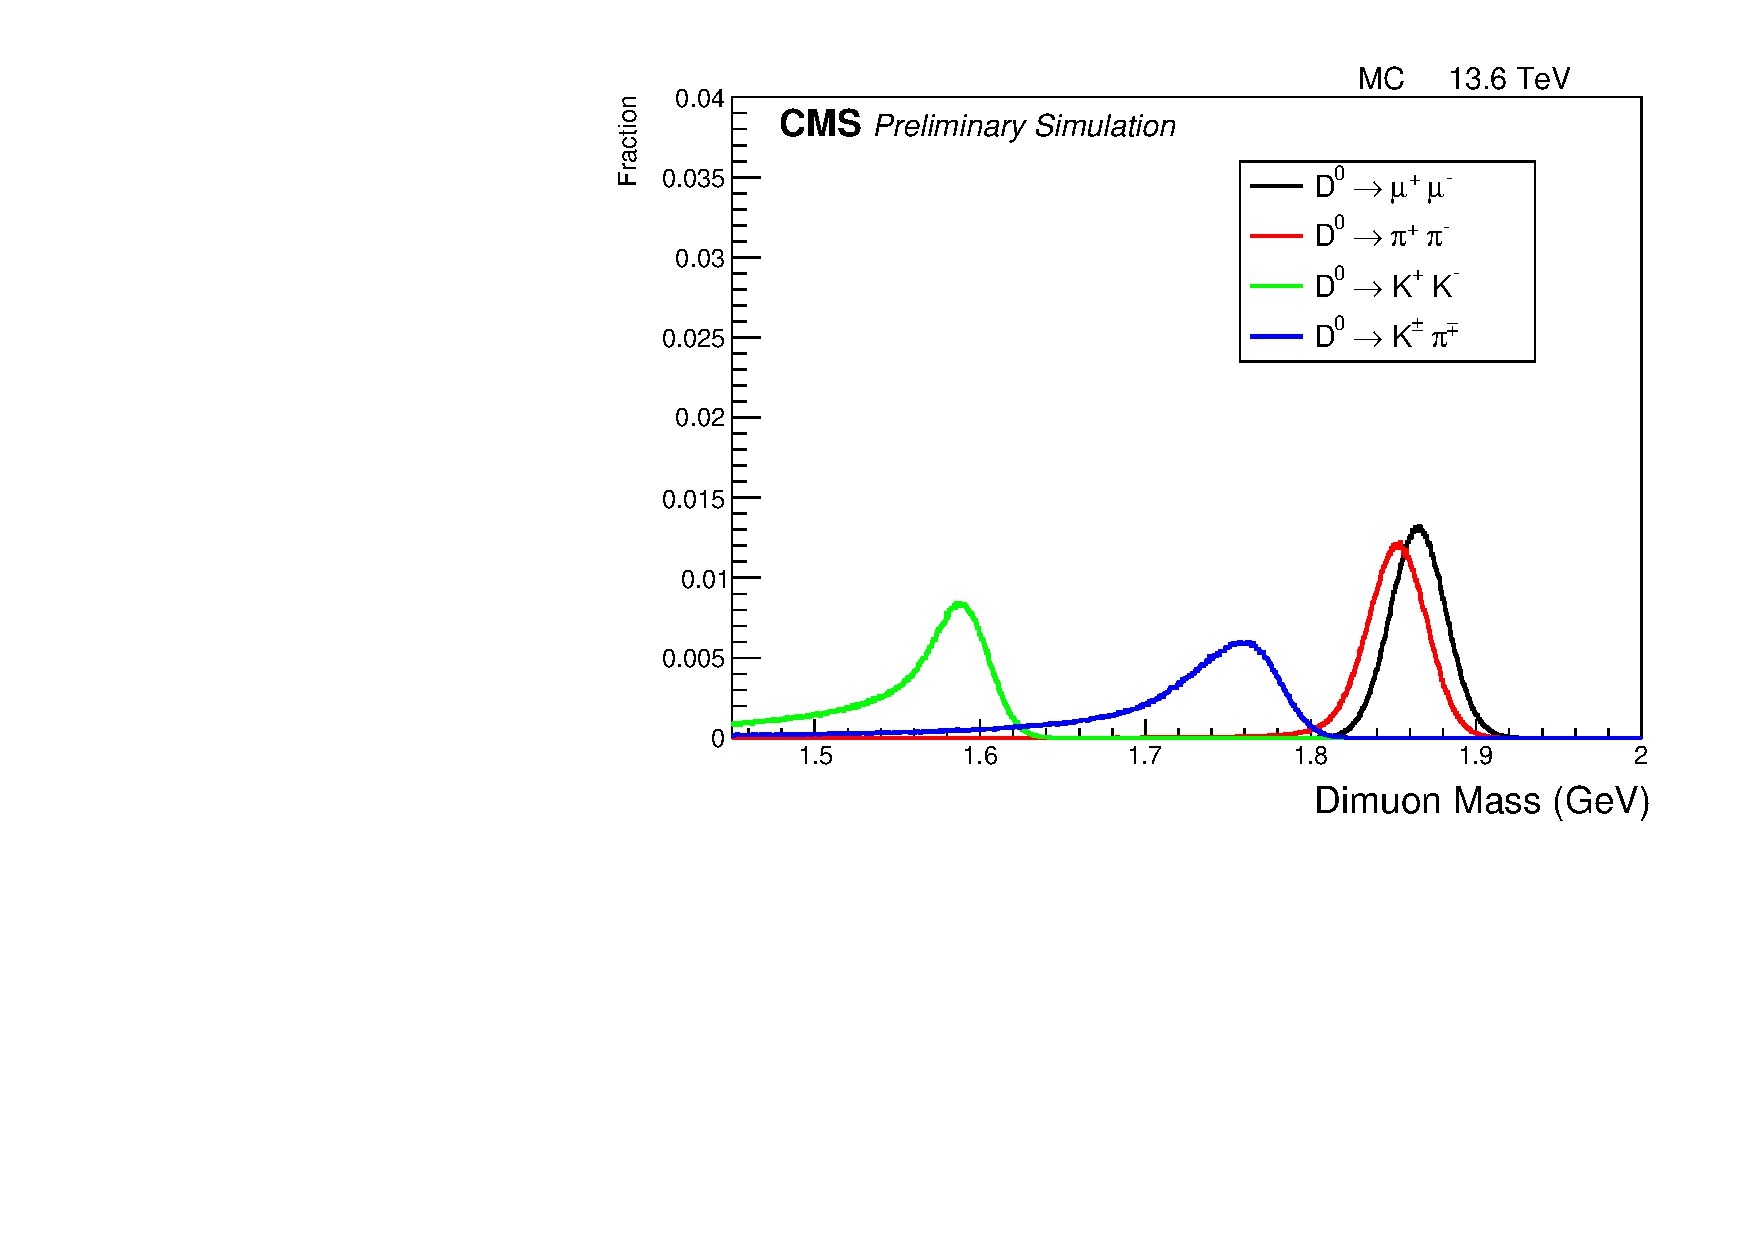
\includegraphics[width=0.45\textwidth]{figures/chapter4/reconstructed_D0_mass.pdf}
      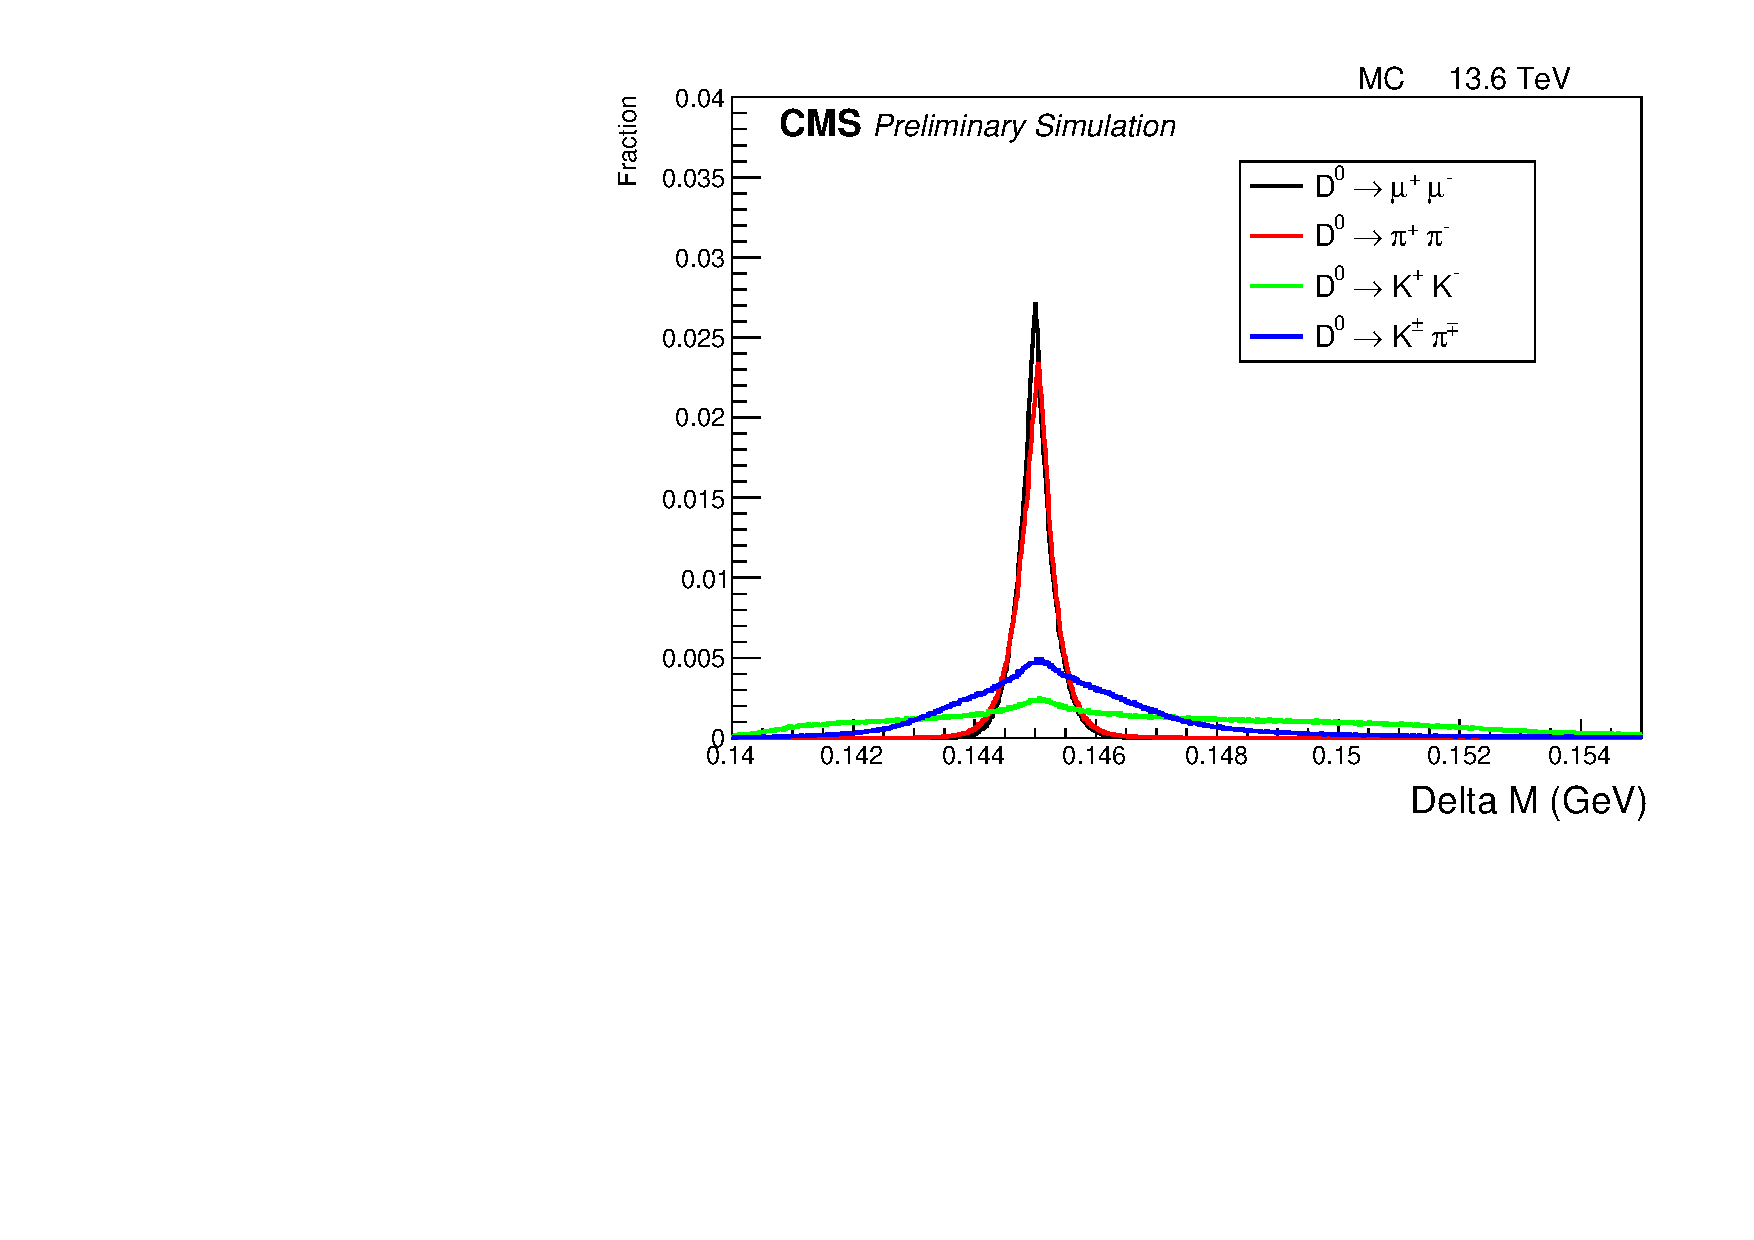
\includegraphics[width=0.45\textwidth]{figures/chapter4/reconstructed_delta_m.pdf}\\
    \end{center}
    \caption{
      Comparison of normalized frequencies for various peaking background $D^0 \to \mu^+ \mu^-$ decays against the signal decay.
      Right: Reconstructed $\Delta m$ distribution.
      Left: Reconstructed dimuon mass distribution, where decay products are forced to take the muon mass using \texttt{TGenPhaseSpace}, even for non-dimuon final states.
    }
    \label{fig:reconstructed_D0_comparison}
  \end{figure}
  
  


\subsection{Monte Carlo samples}

The main component of constructing the Monte Carlo (MC)simulation samples is properly modeling the $D^*$ meson by replicating their production in the CMS detector. The $D^*$ has two primary production mechanisms at the LHC
\begin{enumerate}
    \item Production through hadronization of charm quark directly from the proton-proton collision, creating prompt $D^*$ mesons close to the primary vertex. 
    \item Production through decay of other hadrons, most commonly the $B$ meson, creating displaced $D^*$ mesons from a secondary vertex
\end{enumerate}

It is important to model both of these production mechanisms of the $D^*$ decay to generate a reliable MC simulation sample. Specifically, the first method produces a prompt soft pion in the $D^*\pm \to D^0 \pi^\pm$ process while the second method produces a displaced soft pion, resulting in significant differences in vertex parameters used in reconstruction and classification. Therefore, over 200 seperate MC samples are produced for this analysis. Their full complexity extends beyond the scope of this thesis, but table \ref{tab:mc-samples} displays some of the most used samples.

\begin{tabularx}{\textwidth}{|l|X|}
    \hline
    \textbf{Sample Name} & \textbf{Attributes} \\
    \hline
    DstarToD0Pi\_D0To2Mu\_MuFilter &
    \begin{itemize}
      \item SoftQCD:nonDiffractive (MinBias)
      \item force $D^* \to D^0\pi$, $D^0 \to \mu^+\mu^-$ decay
      \item $|\eta(D^*)| < 3.0$
      \item $|\eta(D^0)| < 3.0$ for $D^0$ originating from $D^*$
      \item $|\eta| < 2.6$, $p_T > 3.0$ for muons originating from $D^0$
    \end{itemize} \\
    \hline
    DstarToD0Pi\_D0To2Pi\_PiFilter &
    \begin{itemize}
      \item SoftQCD:nonDiffractive (MinBias)
      \item force $D^* \to D^0\pi$, $D^0 \to \pi^+\pi^-$ decay
      \item $|\eta(D^*)| < 3.0$
      \item $|\eta(D^0)| < 3.0$ for $D^0$ originating from $D^*$
      \item $|\eta| < 2.6$, $p_T > 3.0$ for pions originating from $D^0$
    \end{itemize} \\
    \hline
    DstarToD0Pi\_D0ToKPi\_KPiFilter &
    \begin{itemize}
      \item SoftQCD:nonDiffractive (MinBias)
      \item force $D^* \to D^0\pi$, $D^0 \to K^-\pi^+$ decay
      \item $|\eta(D^*)| < 3.0$
      \item $|\eta(D^0)| < 3.0$ for $D^0$ originating from $D^*$
      \item $|\eta| < 2.6$, $p_T > 3.0$ for pions originating from $D^0$
    \end{itemize} \\
    \hline
    DstarToD0Pi\_D0To2Pi\_PiToMuPiFilter\_PiLifetime0p02 &
    \begin{itemize}
      \item SoftQCD:nonDiffractive (MinBias)
      \item force $D^* \to D^0\pi$, $D^0 \to \pi^+\pi^- \to \mu^+\nu_\mu\mu^-\nu_\mu$ decay
      \item reduced lifetime for charged pions by a factor of 50 from $c\tau = 7.8\,\text{m}$ to $c\tau = 15.6\,\text{cm}$
      \item pion decay limits: $R < 2$ m, $|z| < 4$ m
      \item $|\eta(D^*)| < 3.0$
      \item $|\eta(D^0)| < 3.0$ for $D^0$ originating from $D^*$
      \item $|\eta| < 2.6$, $p_T > 3.0$ for pions originating from $D^0$
      \item $|\eta| < 2.6$, $p_T(\mu) > 3.0$ for muons originated from charged pions
    \end{itemize} \\
    \hline
\end{tabularx}

TODO: fix this table

\section{Selections and efficiency}

Once we've attained the data and monte carlo samples needed for this analysis, we filter through them using event selections, carefully tracking the \textit{acceptance} and \textit{efficiency} for each selection\footnote{We define \textit{acceptance} as TODO and \textit{efficiency} as TODO}. The selection process can be broken down into three main stages:
\begin{enumerate}
    \item The \textit{preselection} stage provides the selections which are tied to trigger requirements, reconstruction requirements, and dataset size limitations.
    \item The \textit{baseline selection} stage primarily is used to reject background samples while keeping the efficiency high, the sidebands of the signal region large, and the signal shape unperturned. 
    \item The \textit{multivariate analysis (MVA) selection} stage uses ML-methods to optimize the background rejection.
\end{enumerate}

\subsection{Preselection}
\label{subsec:preselection}

The preselection is used to create reconstructed event candidates which pass the triggers discussed in section TODO. To stay consistent between signal and normalization events, we keep a similar preselection process for both $D^{*\pm} \to D^0 \pi^\pm, D^0 \to \mu^+ \mu^-$ and $D^{*\pm} \to D^0 \pi^\pm, D^0 \to \pi^+ \pi^-$ events.

In order to properly reconstruct the $D^{*\pm} \to D^0 \pi^\pm, D^0 \to \mu^+ \mu^-$ and $D^{*\pm} \to D^0 \pi^\pm, D^0 \to \pi^+ \pi^-$ events, we first must reconstruct their decay products: the muons and pion. Pions are reconstructed from charged tracks found in the tracker. These track are reconstructed using particle flow (PF) algorithms\footnote{The primary goal of these algorithms is to reconstruct individual particles using the data read out from the detector itself. This is made especially difficult because of the high lumonisties of run3 resulting in a large amount of \textit{pileup}, a phenomenon that occurs due to multiple proton-proton collisions happening within a very short time frame resulting in multiple collisons per event. }, meaning the pions used in the analysis are labeled as PF candidates. Muons are reconstructed primarily using detector read out from the muon chambers. We use the well established CMS reconstruction algorithms \texttt{TrackerMuon} and \texttt{GlobaleMuon} as well as use the collaboration's \texttt{LooseMuonID} for muon identification. To reduce background noise and increase detector resolution, we also cut at $p_T>4$ GeV and require a \texttt{highPurity} inner track in the tracker for both pions and muons.

Once we have the muon and/or pion candidates for the $D^0$ decay, we use vertex reconstruction to reconstruct the full decay candidate. A \textit{vertex} is the location in 3D space where a process occured and the \textit{primary vertex} is the location of the interaction of the quarks of the two colliding protons, which in our case produce the $D^{*\pm}$. Due to the short mean lifetime of the $D^{*\pm}$ ($ 6.9 \pm 1.9 \times 10^{-21} \; s$) \cite{ref:pdg2024}, we can label the $D^{*\pm} \to D^0 \pi^\pm$ vertex using the primary vertex. The kinematic vertex reconstruction begins by identifying the dimuon or dipion decay candidates (i.e two pions or two muons which came from the same decay). The two 4-momentum vectors of these two candidates is added together to get a dimuon or dipion 4-momentum vector. We call this dimuon/dipion system a $D^0$ candidate. Using the $D^0$ candidate 4-momentum vector, we calculate the transverse momentum of $D^0$ candidate and extrapolate it to its intersection with the beamline. Then, in order to determine which primary vertex\footnote{There are often many primary vertices in one event due to pileup} the $D^{*\pm} \to D^0 \pi^\pm$ decay came from, we calculate the 3D distance between each primary vertex candidate and the extrapolated intersection point, known as the \textit{3D-impact parameter}, and find the primary vertex which minimizes this parameter. Lastly, since the decay at the primary vertex is $D^{*\pm} \to D^0 \pi^\pm$, we check if there exists a soft pion which came from the selected primary vertex. This kinematic vertex reconstruction is then used to gather reconstructed signal and normalization events as well as refit the $D^0$ candidates to a common vertex using a kinematic vertex fitting tool (TODO: insert citation), generating \textit{refitted} candidates. The events which pass this reconstruction are thus the events that pass the preselection. 

\begin{figure}[htbp]
    \centering
    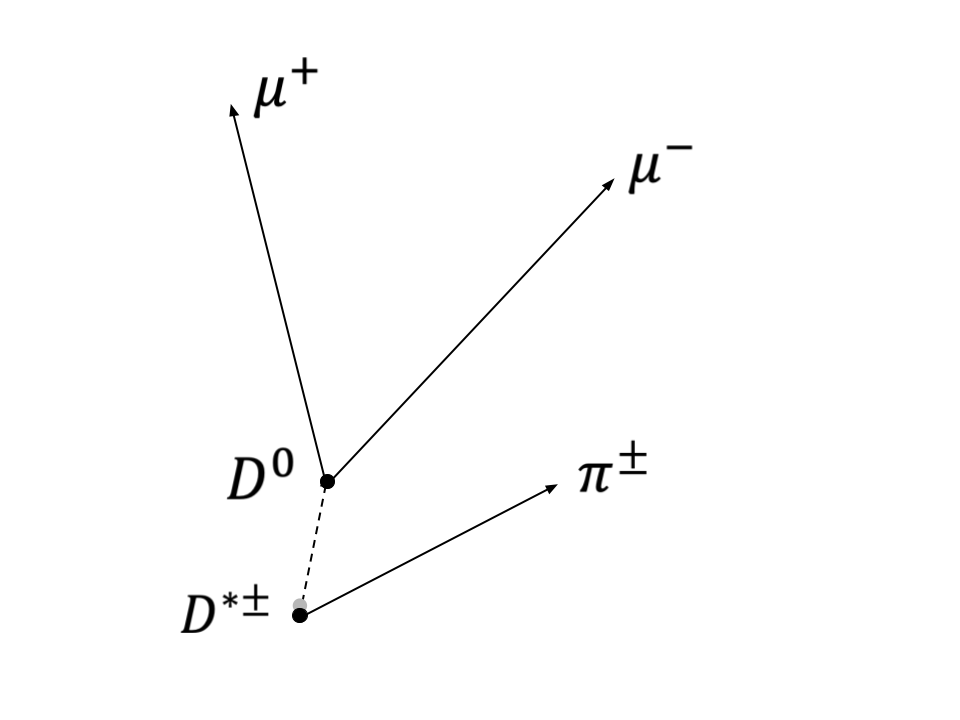
\includegraphics[width=0.8\textwidth]{figures/chapter4/vertex_reconstruction.png}
    \caption{An example of the $D^{*\pm} \to D^0 \pi^\pm, D^0 \to \mu^+ \mu^-$ vertex}
    \label{fig:vertex_reconstruction}
\end{figure}

\subsection{Baseline selection}
\label{subsec:baseline_selection}

Using the reconstruction described in section \ref{subsec:preselection}, we are able to extract several kinematic variables from $D^{*\pm} \to D^0 \pi^\pm$ candidates outputted by the preselection. These variables are used in the baseline selection as well as in other parts of the analysis. They are defined here as follows:
\begin{enumerate}
    \item Reconstructed $D^0$ mass: the mass calculated from from the addition of the two 4-momentum vectors of the $D^0$'s product candidates (either dimuon or dipion). 
    \item Refitted $D^0$ mass: the mass calculated from from the addition of the two 4-momentum vectors of the $D^0$'s product candidates (either dimuon or dipion) once they have been refitted using the kinematic vertex fitting. 
    \item Reconstructed $\Delta m$: the mass difference between the reconstructed $D^{*\pm}$ candidates and the reconstructed $D^0$ candidates. 
    \item Refitted $\Delta m$: the mass difference between the $D^{*\pm}$ and the $D^0$ candidates once they have been refitted using the kinematic vertex fitting.
    \item $\delta_{3D}$: the 3D impact parameter as defined in section \ref{subsec:preselection})
    \item $\delta_{3D}/\sigma\left(\delta_{3D}\right)$: the significance of the 3D impact parameter. This is calculated by taking the value of the 3D impact parameter and dividing it by the square root of the expected variance of the parameter. 
    \item $l_{3D}$: the 3D distance between the vertex of the $D^{*\pm} \to D^0 \pi^\pm$ decay (primary vertex) and the vertex of the $D^0 \to l l$ decay. This can also be called the $\textit{flight length}$ of the $D^0$ meson. 
    \item $l_{3D}/\sigma\left(l_{3D}\right)$: the significance of the 3D distance between the vertex of the $D^{*\pm} \to D^0 \pi^\pm$ decay (primary vertex) and the vertex of the $D^0 \to l l$ decay. Calculated by taking the value of the distance and dividing it by the square root of the expected variance of the distance. 
    \item $l_{xy}$: the distance in the $xy$ plane (perpendicular to the beam line) between the vertex of the $D^{*\pm} \to D^0 \pi^\pm$ decay (primary vertex) and the vertex of the $D^0 \to l l$ decay.  This can also be called the $\textit{transverse flight length}$ of the $D^0$ meson. 
    \item $l_{xy}/\sigma\left(l_{xy}\right)$: the significance of the distance in the $xy$ plane between the vertex of the $D^{*\pm} \to D^0 \pi^\pm$ decay (primary vertex) and the vertex of the $D^0 \to l l$ decay. Calculated by taking the value of the distance and dividing it by the square root of the expected variance of the distance. 
    \item $\alpha_{3D}$ : the angle between the $D^0$ momentum and flight direction. 
    \item $D^0$ vertex probability: the probability given by the $\chi^2$ fit which reconstructs the $D^0$ vertex 
    \item $D^*$ vertex probability: the probability given by the $\chi^2$ fit which reconstructs the $D^*$ vertex
\end{enumerate}
Note that, unless otherwise stated, the refitted variables are used over the reconstructed ones. 

Using these variables, we impart a baseline selection on the preselected events. The goal of the baseline selection is to reject much of the background while keeping the signal efficiency high and not perturbing the signal shape. To achieve this, we select a $D^0$ reconstructed mass in the range of TODO INSERT RANGE, $D^0$ refitted mass in the range of TODO: INSERT RANGE, reconstructed $\Delta m$ in the range of TODO: INSERT RANGE, and refitted $\Delta m$ in the range TODO: INSERT RANGE. As seen in figure TODO: INSERt FIGURE, these ranges are picked such that there are large sidebands on the signal, keeping signal efficiency high as shown in table: TODO INSERT TABLE.

The other set of baseline selections are on the vertices themselves. We require the $D^*$ vertex probability to be greater that $0.1$ and the $D^0$ vertex probability to be greater than $0.01$. This is done such that there is some confidence in the vertex reconstruction and such that we can match the double muon trigger requirement of $0.005$. To gain further confidence in the vertex reconstruction, we limit $\alpha_{3D} < 0.1$ radians and the flight length significance to be greater than 3. Lastly, to keep the normalization channel (which is gathered from a ZeroBias trigger) under the same selection as the signal channel (which is gather from a HLT\_DoubleMuon trigger), we require the event in the normalization channel to have fired the \texttt{HLT\_DoubleMu4\_3\_LowMass} trigger. Note, this does not mean than the specific decay we reconstruct fired the trigger, in fact usually some other event has fired the trigger. 

TODO: insert figure of variable plots

TODO: insert table of efficiencies


\subsection{Multivariate Analysis}
\label{subsec:mva}

The preselection and baseline selections optimize signal efficiency, but not overall analysis sensitivity. In order to optimize the analysis sensitivity, we train a classifier using a decision tree model driven multivariate analysis (MVA). This single classifying parameter can then be used as a selection parameter named $\text{MVA}_D$ and the cut can be tuned to optimize analysis sensitivity.

The decision tree model used is based on the XGBoost (Extreme Gradient Boosting) library, which builds a forest of regression trees trained sequentially to minimize a regularized objective function. Each tree in the sequence focuses on correcting the erros of the previous tree and the scores from the trees are combined to get a final prediction on the classifiction of the event from the forest. Each tree is constructed using a greedy algorithm that selects splits based on gain, with regularization terms penalizing model complexity to prevent overfitting. The loss function is binary logistic loss, which is optimized using boosting under second-order gradient information with an evaluation metric based on the area under the receiver-operating characteristic (ROC) curve, known as AUC in the literature. Each tree has a maximum depth of 3 and is trained using a learning rate of $\eta = 0.1$. An additional regularization is applied with an L1 penalty. A minimum loss reduction threshold for tree splits\footnote{This requirement only allows additional trees to form if their contribution causes the loss to decrease by some number, set in this analysis to be $2.0$} and a sub-sample ratio\footnote{This is the fraction of training data that each tree sees, which for this analysis is kept (as is standard) at $60\%$} are employed to additionally prevent overfitting. The model is trained for over 4000 epochs in each training round.

The signal events used for training are taken from simulated $D^0 \to \mu^+ \mu^-$ MC samples. The background events are taken from the data sidebands using the $\delta M$ parameter with a distance of over $5\sigma$ right of the expected value ($\delta m \in [0.150, 0.155]$ GeV) and dimuon mass in the signal range of $[1.81, 2.45]$ GeV. The dimuon mass is kept in the signal range to align the training data with not obviously rejected events. Should the background training data be selected outside the signal dimuon mass window, the classification of signal and background events would become trivial, leading to a less effective model.

The variables used in the training are
\begin{enumerate}
    \item The $p_T$ of both muons and the soft pion
    \item The $D^0$ vertex parameters, including point angle, flight length significance, vertex probability, 3D impact parameter, and significance of the 3D impact parameter.
    \item The $D^*$ vertex probability.
    \item The $D^0$ mass resolution over the $D^0$ mass.
\end{enumerate}

\begin{figure}[htp]
    \begin{center}
      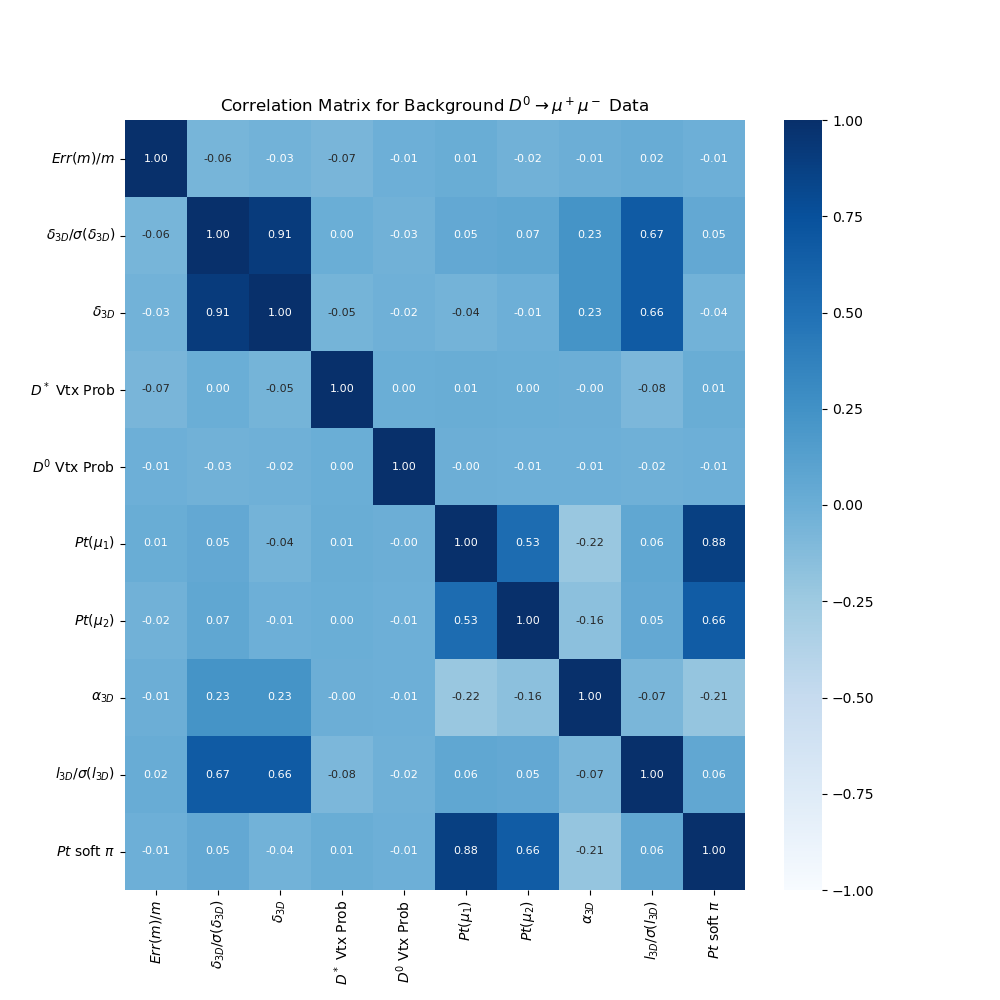
\includegraphics[width=0.45\textwidth]{figures/chapter4/mva/Correlation_data.png}
      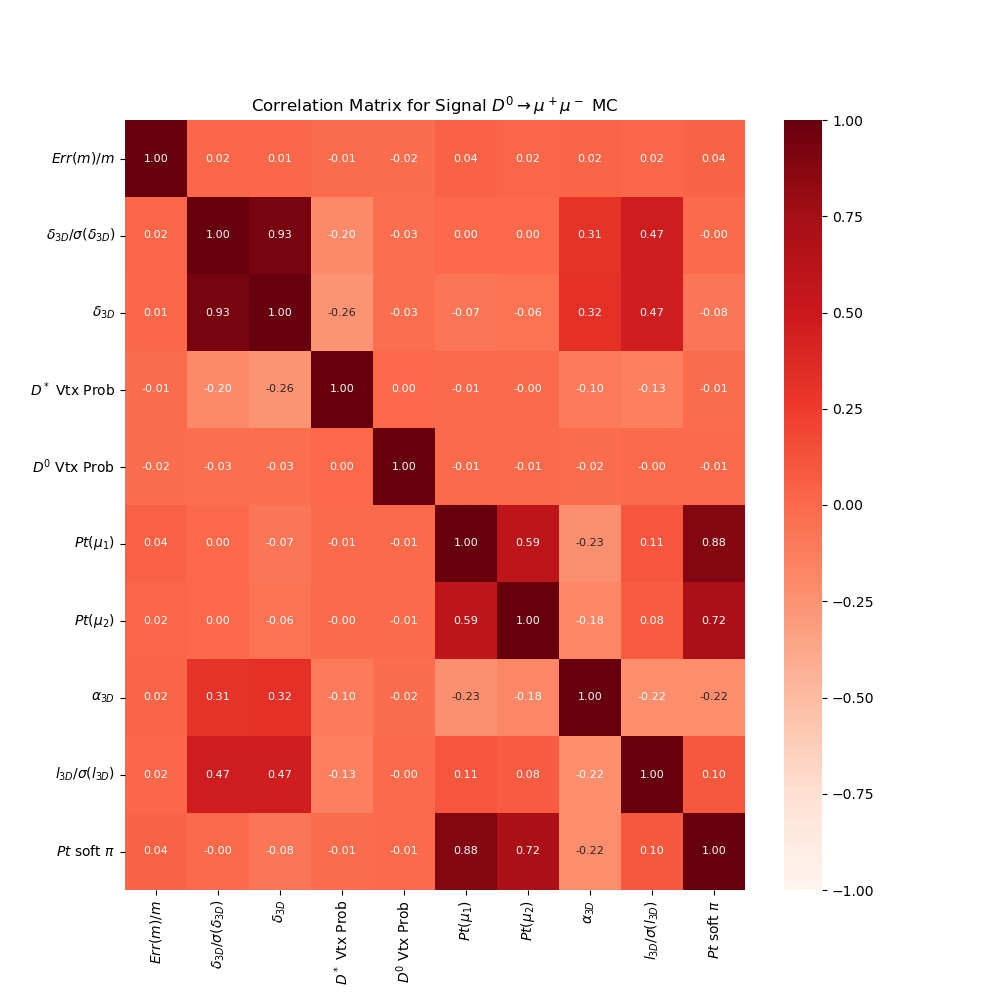
\includegraphics[width=0.45\textwidth]{figures/chapter4/mva/Correlation_dmm.png}\\
    \end{center}
    \caption{
      Correlation matrix over the MVA training variables for training background events generated from data (left) and training signal events generated from MC (right)
    }
    \label{fig:mva_correlation_matrix_for_training_variables}
\end{figure}

The correlation matrix for both the signal and background can be seen in figure \ref{fig:mva_correlation_matrix}. Importantly, there are some positive correlation between features and there are no two strong anti-correlated features, meaning we expect stability in learning due to feature redundancy and simpler interactions, yet expect good model generalization. 

Due to the relatively small amount of data avilable, the data is split into 5 groups and 5 seperate models are training, each using a different data group as testing data sets and the remaining 4 as training datasets. This ensures the models have been exposed on the entire dataset while not overfitting on any particular events. Once the models have been trained, the event number (which is independent of the contents of the event), is used to decide which model to use for classification of that event. 

It is important that the classification parameter is not correlated with any variables used later in the analysis for fitting (namely $\delta M$ and the dimuon mass) so as to not skew the fit. Due to this, the kinematic variable given to the model are restricted to $p_T$ and vertex parameters, so that it is not possible to reconstruct masses. To check that the correlations don't exist, a correlation matrix between the classification parameter, $\delta M$, and the dimuon mass is created and shown in figure \ref{fig:mva_correlation_matrix_for_fit_variables}. As expected, there is no correlation.


\begin{figure}[htp]
    \begin{center}
      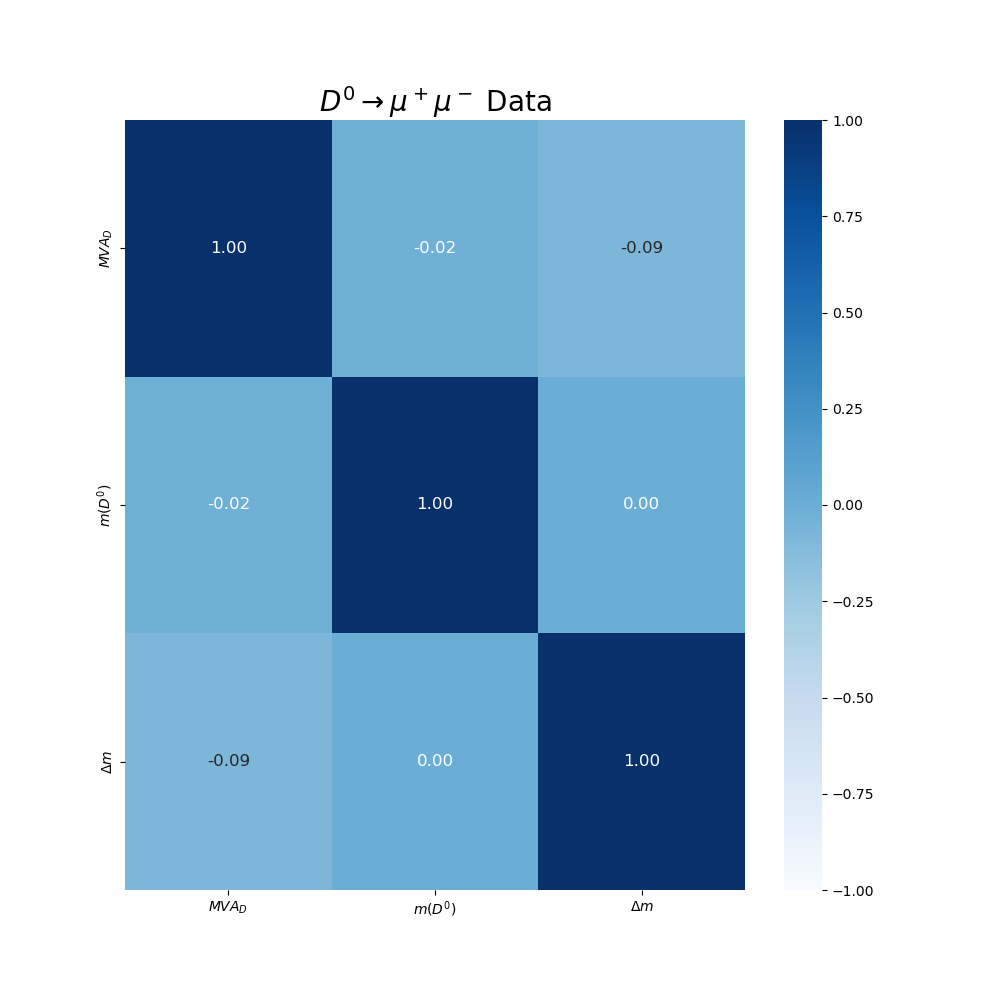
\includegraphics[width=0.45\textwidth]{figures/chapter4/mva/Correlation_data_obs.png}
      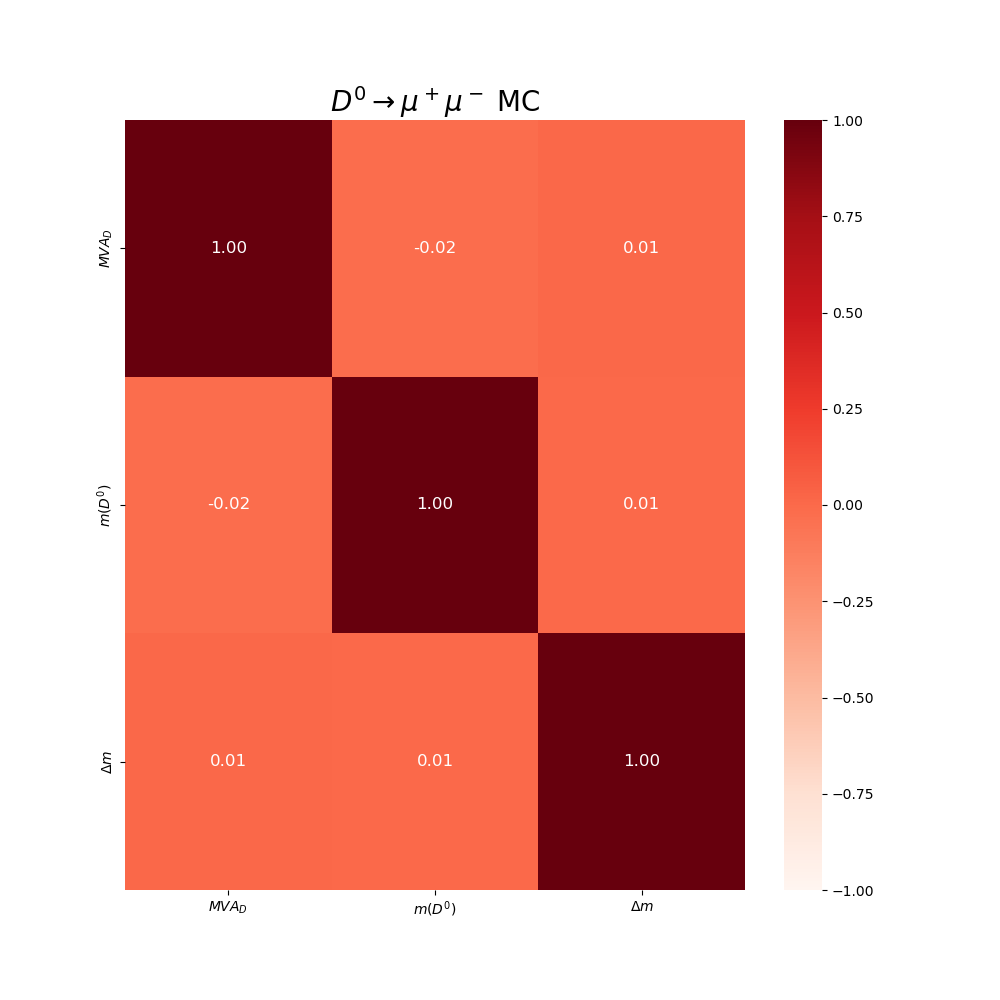
\includegraphics[width=0.45\textwidth]{figures/chapter4/mva/Correlation_dmm_obs.png}\\
    \end{center}
    \caption{
      Correlation matrix comparing the MVA classification parameter to $\delta M$ and the dimuon mass. Shown left is the training background events generated from data and shown right is the training signal events generated from MC.
    }
    \label{fig:mva_correlation_matrix_for_fit_variables}
\end{figure}

It is also important to note that the classifier is being trained and tested on simulated signal samples, yet for the analysis the efficiency of the classifier on real data is needed. Due to mismodeling effect in the simulation, the simulation efficiency is not necessarily the same as the data efficiency. Getting the efficiency is difficult to measure directly since the expected branching fraction of $D^0 \to \mu^+ \mu^-$ is so low that we do not have a reliable data sample for the signal. Instead, the efficiency is derived from the $D^0 \to \pi^+ \pi^-$ decay using the zero bias dataset and the $D^0 \to \pi^+ \pi^-$ monte-carlo simulation samples. Since the $D^0 \to \pi^+ \pi^-$ decay behaves similarly to the $D^0 \to \mu^+ \mu^-$ decay in terms of reconstruction/vertex parameters and the MVA classifier is independent of $\delta M$ and dimuon mass in both cases, the efficiency derived from $D^0 \to \pi^+ \pi^-$ is similar to the efficiency of $D^0 \to \mu^+ \mu^-$. Therefore, the same classifier with the same cut is used on both the normalization channel and the signal channel, causing the efficiencies to cancel in the branching fraction equation. TODO: link equation. We calculate the efficiency in data on the $D^0 \to \pi^+ \pi^-$ decay by performing the UML fit outlined in section TODO: (insert section link) on different $\text{MVA}_D$ cut values and comparing to the \texttt{ZeroBias} dataset. In simulated data, we are able to directly tag the signal events that were created from the simulation, so calculating the efficiency is trivial. A list of efficency values at specific $\text{MVA}_D$ cuts can be found in table \ref{tab:mva_cut_efficiencies} and a graphical representation over a more diverse $\text{MVA}_D$ cut range can be found in \ref{fig:mva_cut_efficiencies}.

\begin{table}[htbp]
    \centering
    \begin{tabular}{|l|c|c|c|}
    \hline
    $\text{MVA}_D$ cut value & \textbf{0.74} & \textbf{0.76} & \textbf{0.78} \\
    \hline
    $D^0 \to \pi^+ \pi^-$ Data Efficiency (from Zero Bias) & $0.722 \pm 0.088$ & $0.707 \pm 0.087$ & $0.681 \pm 0.086$ \\
    $D^0 \to \pi^+ \pi^-$ MC Efficiency & 0.817 & 0.801 & 0.783 \\
    $D^0 \to \mu^+ \mu^-$ MC Efficiency & 0.824 & 0.809 & 0.792 \\
    $D^0 \to \mu^+\nu_\mu\mu^-\bar{\nu}_\mu$ MC Efficiency & 0.806 & - & - \\
    \hline
    \end{tabular}
    \caption{Summary of $\text{MVA}_D$ cut efficiency at various cut values on various samples used throughout the analysis.}
    \label{tab:mva_cut_efficiencies}
\end{table}

\begin{figure}[htp]
    \begin{center}
      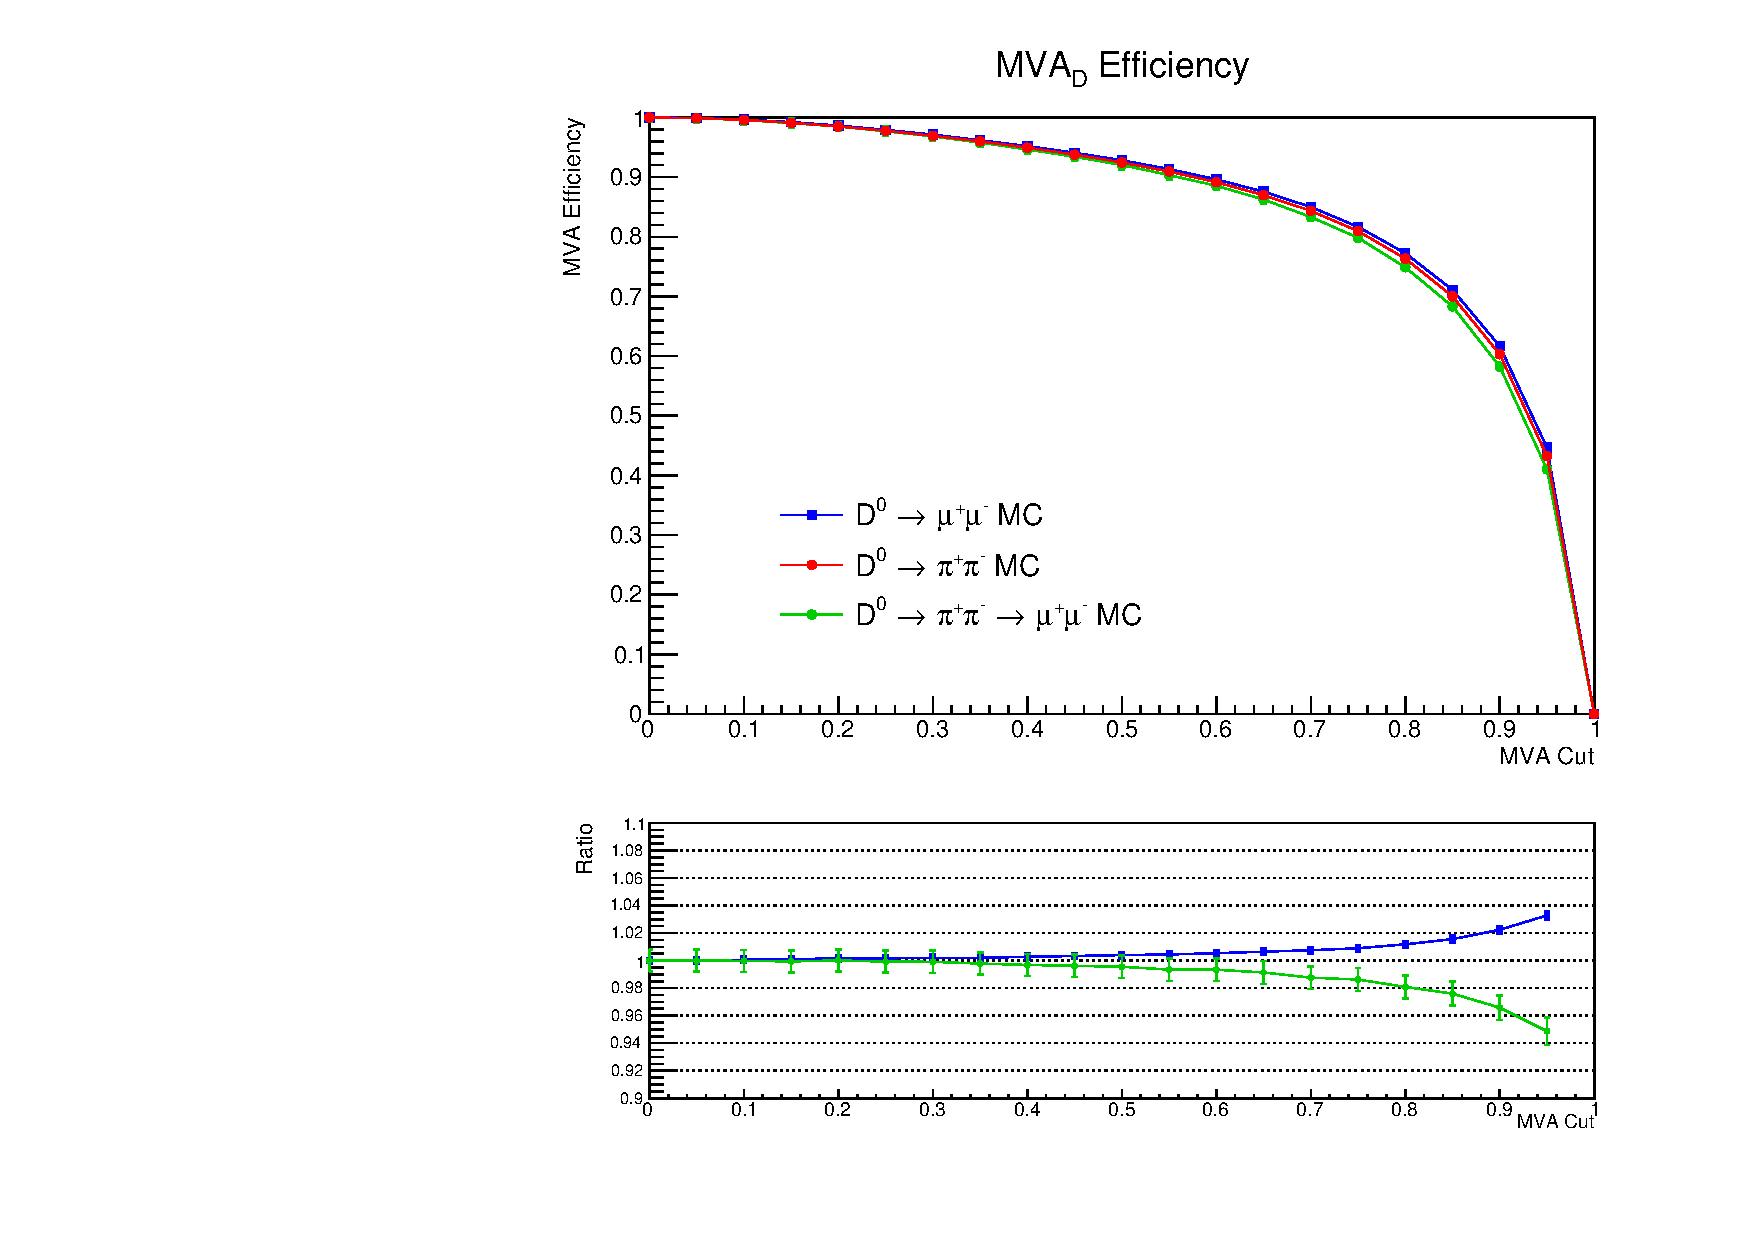
\includegraphics[width=0.5\textwidth]{figures/chapter4/mva/mva_efficiency.pdf}
    \end{center}
    \caption{
      A graphical summary of $\text{MVA}_D$ cut efficiency at various diverse cut values on various samples used throughout the analysis.
    }
    \label{fig:mva_cut_efficiencies}
\end{figure}

As can be seen in table \ref{tab:mva_cut_efficiencies} as well as figure \ref{fig:mva_cut_efficiencies}, while the efficiency values are, as expected, extremely close in the MC samples, there is still a small difference between the three decay channels. To account for this small difference, we calculate a corrective efficiency factor, derived from Monte Carlo. We name this corrective factor $\text{MVA}_{D, cor}$ and define it as
\begin{equation}
    \begin{split}
    \text{MVA}_{D,\text{cor}\;(D^0 \to \mu^+ \mu^-)} &= 
    \frac{\epsilon_{D^0 \to \mu^+ \mu^-\; \text{ (simulation)}}}
         {\epsilon_{D^0 \to \pi^+ \pi^-\; \text{ (simulation)}}} \\
    \text{MVA}_{D,\text{cor}\;(D^0 \to \pi^+ \pi^- \to \mu^+ \nu_\mu \mu^- \nu_\mu)} &= 
    \frac{\epsilon_{D^0 \to \pi^+ \pi^- \to \mu^+ \nu_\mu \mu^- \nu_\mu\; \text{ (simulation)}}}
         {\epsilon_{D^0 \to \pi^+ \pi^-\; \text{ (simulation)}}}
    \end{split}
\end{equation}
From these definitions, one can extrapolate to data due to the proximity of the efficiency values, meaning
\begin{equation}
    \begin{split}
    \epsilon_{D^0 \to \mu^+ \mu^-} \text{ (data)} &= 
    \epsilon_{D^0 \to \pi^+ \pi^-} \text{ (data)} 
    \times \text{MVA}_{D,\text{cor}\;(D^0 \to \mu^+ \mu^-)} \\
    \epsilon_{D^0 \to \pi^+ \pi^- \to \mu^+ \nu_\mu \mu^- \nu_\mu} \text{ (data)} &= 
    \epsilon_{D^0 \to \pi^+ \pi^-} \text{ (data)} 
    \times \text{MVA}_{D,\text{cor}\;(D^0 \to \pi^+ \pi^- \to \mu^+ \nu_\mu \mu^- \nu_\mu)}
    \end{split}
\end{equation}
Lastly, a very conservative systematic error is assigned to the $\text{MVA}_{D, cor}$ factors of $|1-\text{MVA}_{D, cor}|$. Therefore, we get
\begin{equation}
\begin{split}
    \text{MVA}_{D,\text{cor}\;(D^0 \to \mu^+ \mu^-)} &= 1.009\;\pm\;0.012 \; \text{(stat)}\;\pm\;0.009 \; \text{(sys)} \\
    \text{MVA}_{D,\text{cor}\;(D^0 \to \pi^+ \pi^- \to \mu^+ \nu_\mu \mu^- \nu_\mu)} &= 0.987\;\pm\;0.020 \; \text{(stat)}\;\pm\;0.013 \; \text{(sys)}
\end{split}
\end{equation}
    
\section{Unbinned Maximum Likelihood Fits}

Now that we have given accurate descriptions of the datasets and selection processes used in this analysis, we are now ready to extract the two main values needed for this analysis, the number of $D^0 \to \pi^+ \pi^-$ events, denoted $N_{D^0 \to \pi^+ \pi^-}$, the number of $D^0 \to \mu^+ \mu^-$ events, denoted $N_{D^0 \to \mu^+ \mu^-}$.

In order to do this, we perform two unbinned maximum likelihood (UML) fits on the events in our data that passes the preselection, baseline selection, and MVA selection processes. Maximum likelihood (ML) fits are statistical methods used to estimated parameters of a model given observed data. A ML fit is a UML fit when the data is not binned into a histogram, but rather the exact data values are used. UML fits define a model $f(\vec{x}; \theta, \theta_N)$, which is a PDF over some set of observed variables, $\vec{x}$ and some model parameters $\theta$ and $\vec{\theta}_N$. The goal of a UML fit is to extract a model parameter $\theta$ given some observed data $\vec{x}_1, \vec{x}_2,...,\vec{x}_N$. $\vec{\theta}_N$ are considered nuisance parameters and are important to defining the model, but are not parameters of interest to the analysis. Once a model has been defined, a likelihood is defined as
\begin{equation}
    \mathcal{L}(\theta, \vec{\theta}_N) = \prod^N_{i=1} f(\vec{x}_i; \theta, \vec{\theta}_N)
\end{equation}
In this formulation, the UML fit can be represented as finding $\hat{\theta} \hat{\vec{\theta}_N}= \text{argmax}_{\theta, \vec{\theta}_N} \mathcal{L}(\theta, \vec{\theta}_N)$\footnote{In practice, this isn't quite true. Often in applications with lots of nuisance parameters, UML fits operate using profile likelihoods. However, the point of this discussion is merely an overview of UML and the complexities will be ignored.}. 

In our analysis, $\theta$ is the true number of signal events (in the normalization channel this is $N_{D^0 \to \pi^+ \pi^-}$ and in our signal channel this is $N_{D^0 \to \mu^+ \mu^-}$), $\vec{x}$ is the $\delta M$ and $m(D^0)$ of our data, and $\vec{\theta}_N$ are the variance parameters needed to construct the signal and background PDFs. As can be seen in figure \ref{fig:mva_correlation_matrix_for_fit_variables}, there exists practically no correlation between $\delta M$ and $m(D^0)$. This tells us that the 2D model can be split as a product of 1D models. More specifically, we have that
\begin{equation}
    f(\vec{x}; \theta, \theta_N) = f_{m(D^0)}(m(D^0); \theta, \theta_N) \times f_{\delta m}(\delta m; \theta, \theta_N)
\end{equation}

A more precise discussion of this construction follows in the sections below. For each of the two channels we begin by developing the models for both the signal and the background. Then, we outline the specifics of the fit and any corrections applied to it. Lastly, we outline the results of the fit. 

\subsection{Normalization Channel Fit}
\label{subsec:normalization_channel_fit}

The goal of the normalization channel is to extract $N_{D^0 \to \pi^+ \pi^-}$. This is done using the \texttt{HLT\_ZeroBias} trigger dataset, as is described in section \ref{subsec:data_samples}. Perhaps the largest difficulty of the UML fit on the normalization channel is that the \texttt{HLT\_ZeroBias} trigger dataset does not contain many of the $D^{*\pm}\to D^0 \pi^\pm, D^0 \to \pi^+ \pi^-$ signal events due to the fact that the trigger doesn't filter for a specific signal. The below section, in part, describes in detail how this difficulty is overcome by using MC data to inform the fit and correcting for MC mismodeling effects when needed in the final fit. 

\subsubsection{Signal Model}

The signal model for the normalization channel describes the $\delta M$ and $m(D^0)$ of the $D^{*\pm}\to D^0 \pi^\pm, D^0 \to \pi^+ \pi^-$ decay. As is common to do for masses in signal distributions, the model for $m(D^0)$ is a sum of two Gaussian distributions forced to share a common mean. Similarly, the model for $\delta M$ is a sum of three Gaussian distributions forced to share a common mean.

Due to the small number of signal events in data, the shape (composing of the means and standard deviations) of this model is determined by fits to simulated MC data. This is because the shape will be much more stable in MC compared to data, simply just because there are more samples in MC. Once the shape is found using MC, it is frozen and only the number of events is allowed to float when the fit is applied to data. The signal model fit to MC can be seen in figure \ref{fig:d0pipi_uml_fit_pipi_model}.

\begin{figure}[htp]
    \begin{center}
      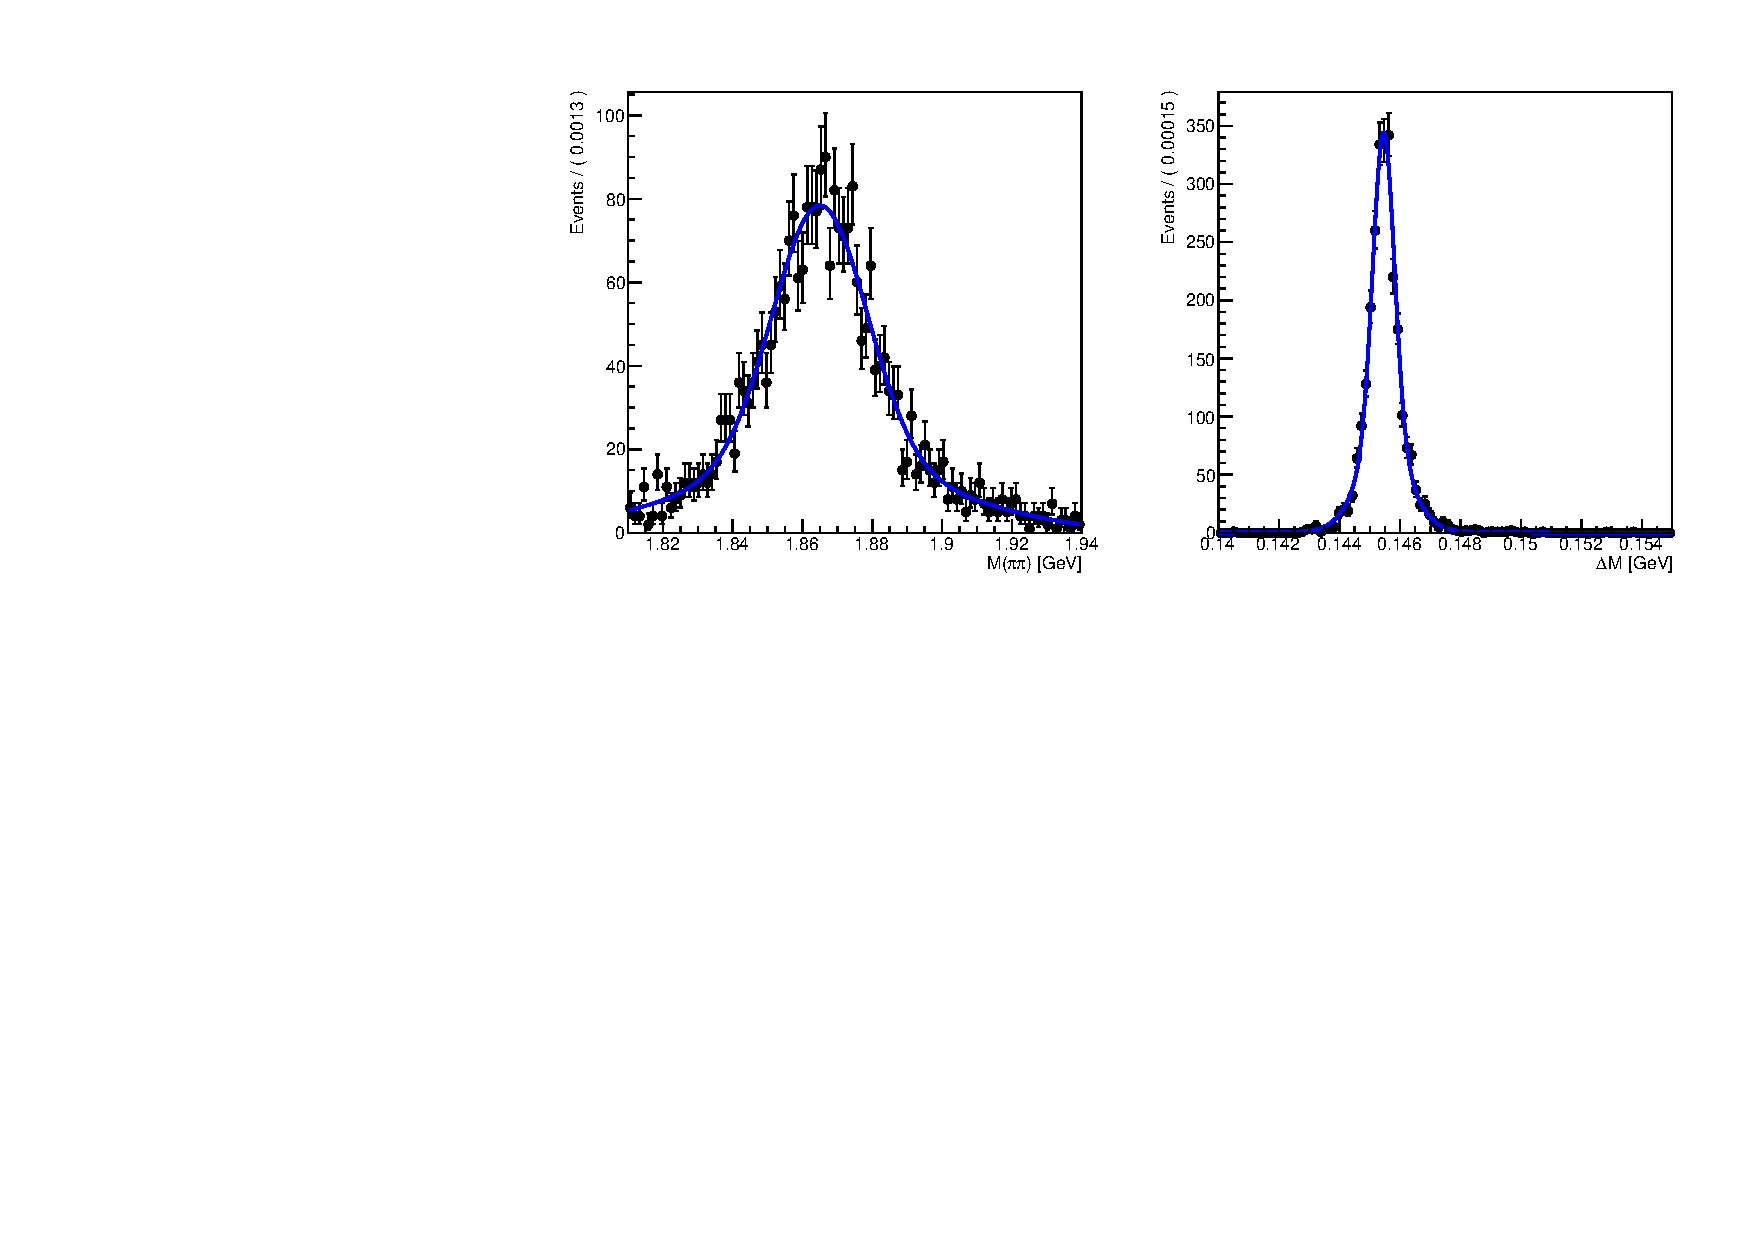
\includegraphics[width=0.9\textwidth]{figures/chapter4/normalization_fit/dpipi_fit_mc.pdf}
    \end{center}
    \caption{
      The signal model fit on MC samples, with $m(D^0)$ displayed left and $\Delta m$ displayed right.
    }
    \label{fig:d0pipi_uml_fit_pipi_model}
\end{figure}

It is possible, however, that the shape varies slightly between the MC samples and data, due to mismodeling in MC. To account for this slight mismodeling affect, we derive correction factors $\mu_{\text{corr}}$ and $\sigma_{\text{corr}}$ such that
\begin{equation}
\begin{split}
    \mu_{\text{data}} &= \mu_{\text{MC}} \times (1+\mu_{\text{corr}}) \\
    \sigma^i_{\text{data}} &= \sigma_{\text{MC}} \times (1+\sigma_{\text{corr}}) 
\end{split}
\label{eq:shape_correction_definition}
\end{equation}
where $i$ is used to denote that each of the models has multiple width parameters (one for each Gaussian distribution that is summed) but only one mean parameter.

To derive what this correction factor is, we use the \texttt{HLT\_DoubleMu4\_3\_LowMass} trigger to construct a dataset with enough signal samples to construct a reliable data-driven fit shape. We then run the full normalization channel UML fit (including the background models) on this data. Comparing that to the shape obtained from MC, we can easily derive the $\mu_{\text{corr}}$ from equation \ref{eq:shape_correction_definition}. 

Initially, it might seem that one could apply the same procedure to find $\sigma_{\text{corr}}$. However, this dimuon trigger enhances the amount of $b\bar{b}$ production in the sample, which biases the width of the $D^{*\pm}\to D^0 \pi^\pm, D^0 \to \pi^+ \pi^-$ decay. Therefore, one must first properly understand that bias before applying the correction in the same way as the mass was done. To understand the bias effect between the Dimuon and Zerobias triggers, we compare $D^{*\pm}\to D^0 \pi^\pm, D^0 \to K^\pm \pi^\mp$ fits from the Dimuon and Zerobias dataset. This is possible because the Kaon decay mode is much more frequent than the pion decay mode. The fitting process is the same as before and the width correction 
can be obtained as
\begin{equation}
    \begin{split}
        1+\sigma_{\text{corr}} &= \left(1+\sigma_{\text{corr, DoubleMuon}}^{D^0\to\pi^+\pi^-}\right) \\
        &\times \frac{
            1+\sigma_{\text{corr, ZeroBias}}^{D^0\to\pi^\pm\pi^\mp}
        }{
            1+\sigma_{\text{corr, DoubleMuon}}^{D^0\to K^\pm\pi^\mp}
        }
    \end{split}
\end{equation}    
%All of the corrections to the signal shape are summarized TODO: add table reference.

%TODO: add table of width corrections.  Likely won't do this

\subsubsection{Background Model}

As described in section \ref{subsec:backgrounds}, there are 3 peaking backgrounds and a combinatorial background to consider in the normalization channel. 

To begin, we describe the 3 peaking backgrounds. The first, as most prominant, of these three backgrounds is the $D^{*\pm} \to D^0\pi^\pm, D^0 \to K^\pm \pi^\mp$. As shown in figure \ref{fig:reconstructed_D0_comparison}, the $m(D^0)$ peak is shifted signficiantly to the left due to incorrect mass of the pion imposed on the kaon during reconstruction. In fact, the mean in shifted so far that only the tail of the Gaussian distribution persists in the mass region of our fit. Since the tail of a Gaussian distribution is approximately an exponential function, we use an exponential function to fit the $m(D^0)$ parameter. This fit proves to be significantly more stable as the exponential function only has one shape parameter that requires fitting while the Gaussian distribution has two. In contrast, the $\Delta m$ distribution of the $D^{*\pm} \to D^0\pi^\pm, D^0 \to K^\pm \pi^\mp$ decay closely follows the shape of the signal. Therefore, we similarly use a sum of three Gaussian distributions with a common mean do model the $\Delta m$ distribution. The convergence of the fit is verified using MC samples and is displayed in figure \ref{fig:d0pipi_uml_fit_kpi_model}. The data fit remains stable even when these shape parameters are allowed to vary. Therefore, we allow the shape of this peaking background to vary when fit to data. 

\begin{figure}[htp]
    \begin{center}
      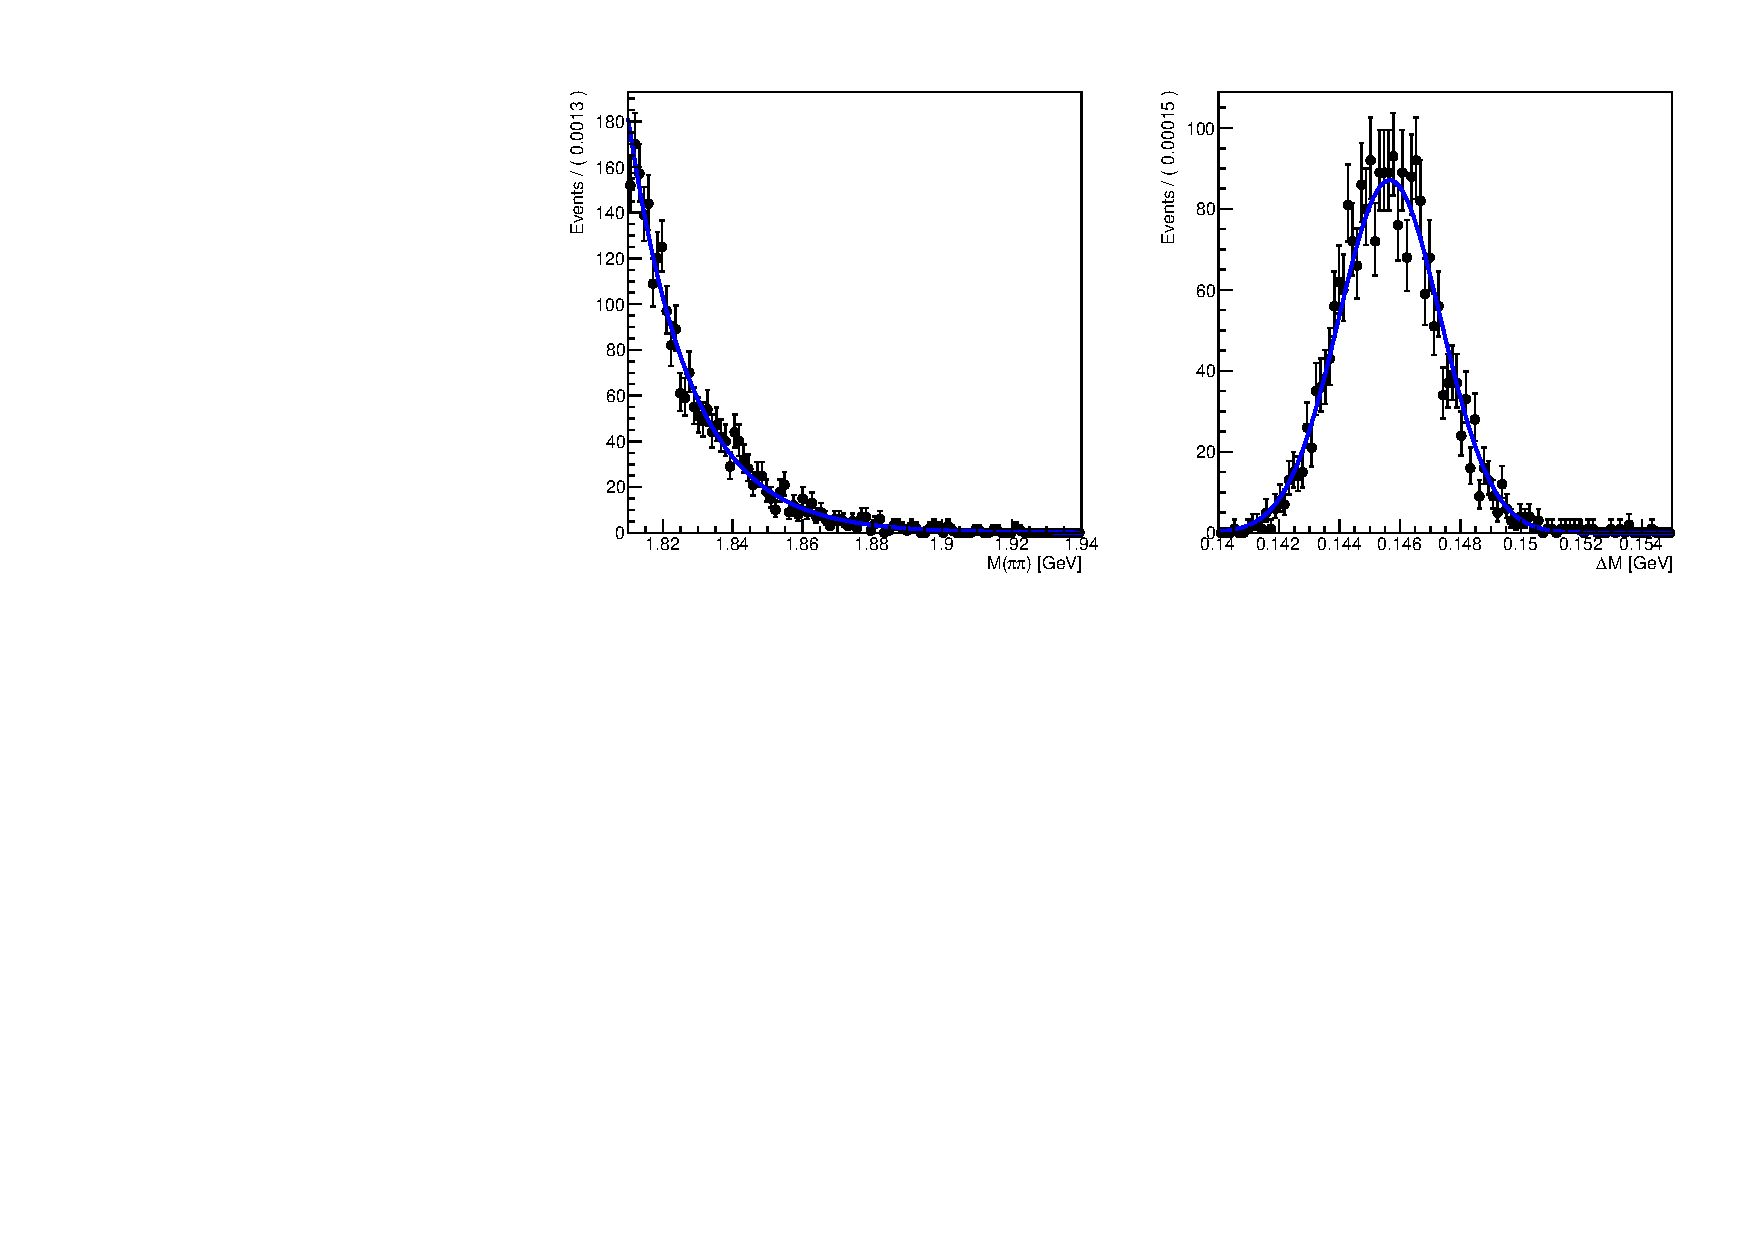
\includegraphics[width=0.9\textwidth]{figures/chapter4/normalization_fit/dpipi_fit_mc_kpi.pdf}
    \end{center}
    \caption{
      The $D^{*\pm} \to D^0\pi^\pm, D^0 \to K^\pm \pi^\mp$ model fit on MC samples, with $m(D^0)$ displayed left and $\Delta m$ displayed right.
    }
    \label{fig:d0pipi_uml_fit_kpi_model}
\end{figure}

The other two peaking backgrounds correspond to $D^0 \to \mu^+ \mu^-$ and $D^0 \to K^\pm \pi^\mp$ decays where the $D^0$ meson does not originate from a $D^*$ meson. Importantly, these have the same $m(D^0)$ shape as their $D^{*\pm} \to D^0 \pi^\pm$ counterparts, so the shape derived from their counterparts is copied exactly into their models. The $\Delta m$ of these decays, however, does not represent a peak but rather a combinatorial signature. This is due to the combinatorial nature of the production mechanisms of the $D^0$ meson that pass the selection criterion. Therefore, we fit a combinatorial background model for the $\Delta m$ values of both non-$D^{*\pm} \to D^0 \pi^\pm$ decays. 

The combinatorial background for $m(D^0)$ is an exponential function, as is common for modeling combinatorial backgrounds of reconstructed rest masses. The combinatorial background for $\Delta m$, however, has more complex shape than just an exponential. In this work, we use the $\texttt{RooDstD0Bg}$ function \cite{ref:verkerke2003roofit} given by
\begin{equation}
    P(m|m_0, A, B, C) = \left(1 - \exp \left(-\frac{m-m_0}{C} \right) \right) \left( \frac{m}{m_0}\right)^A
\end{equation}
The shape of these functions is derived from fits to the data side-band regions where the distance from the signal resonance guarantees virtually no peaking background contribution. This shape is frozen to allow for fit stability when the model is used in the final data fit. Figure \ref{fig:d0pipi_uml_fit_comb_model} shows the convergence of the shape on the data side-bands.

\begin{figure}[htp]
    \begin{center}
      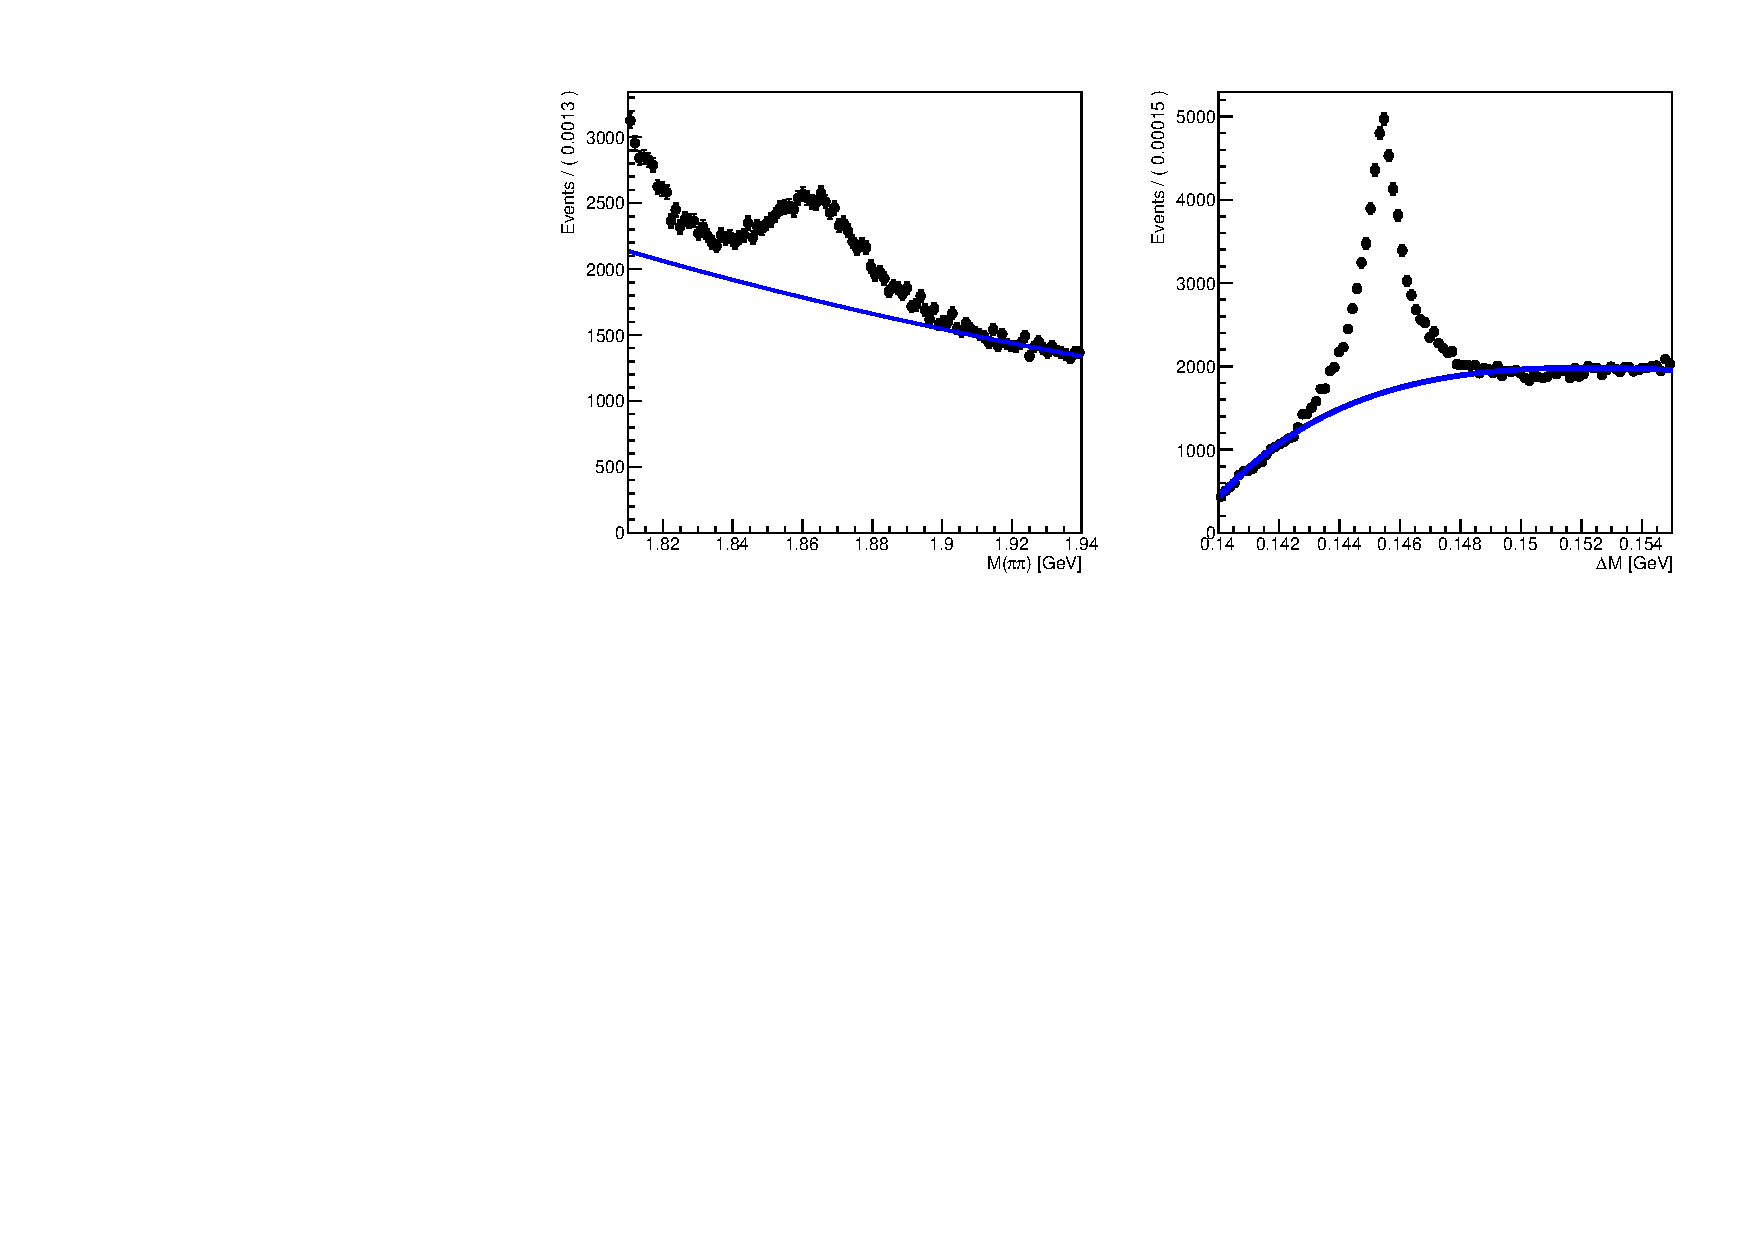
\includegraphics[width=0.9\textwidth]{figures/chapter4/normalization_fit/dpipi_fit_comb.pdf}
    \end{center}
    \caption{
      The combinatorial model fit on data side-bands, with $m(D^0)$ displayed left and $\Delta m$ displayed right.
    }
    \label{fig:d0pipi_uml_fit_comb_model}
\end{figure}

\subsubsection{Fit Results}

The final model used for the fit is a sum of signal model and all the background models. We check the convergence of this model on the \texttt{HLT\_DoubleMu4\_3\_LowMass} data, which contains significantly more signal events than the \texttt{HLT\_ZeroBias} trigger samples, allowing us to visually inspect the stability of the fit, as is seen in figure \ref{fig:d0pipi_uml_fit_dimuon} and table \ref{tab:d0pipi_uml_fit_results}. Importantly, the $D^0 \to K^\pm \pi^\mp$ decays where the $D^0$ meson does not originate from a $D^*$ meson contibutes virtually no events to the fit. Therefore, to increase the stability of the fit, we force the integral under this the non-$D^*,D^0 \to K^\pm \pi^\mp$ model to 0. 

Finally, the fit is applied to the \texttt{HLT\_ZeroBias} trigger samples. A graphical representation of the fit can be seen in figure \ref{fig:d0pipi_uml_fit} and the results are summarized in table \ref{tab:d0pipi_uml_fit_results}.


\begin{figure}[htp]
    \begin{center}
      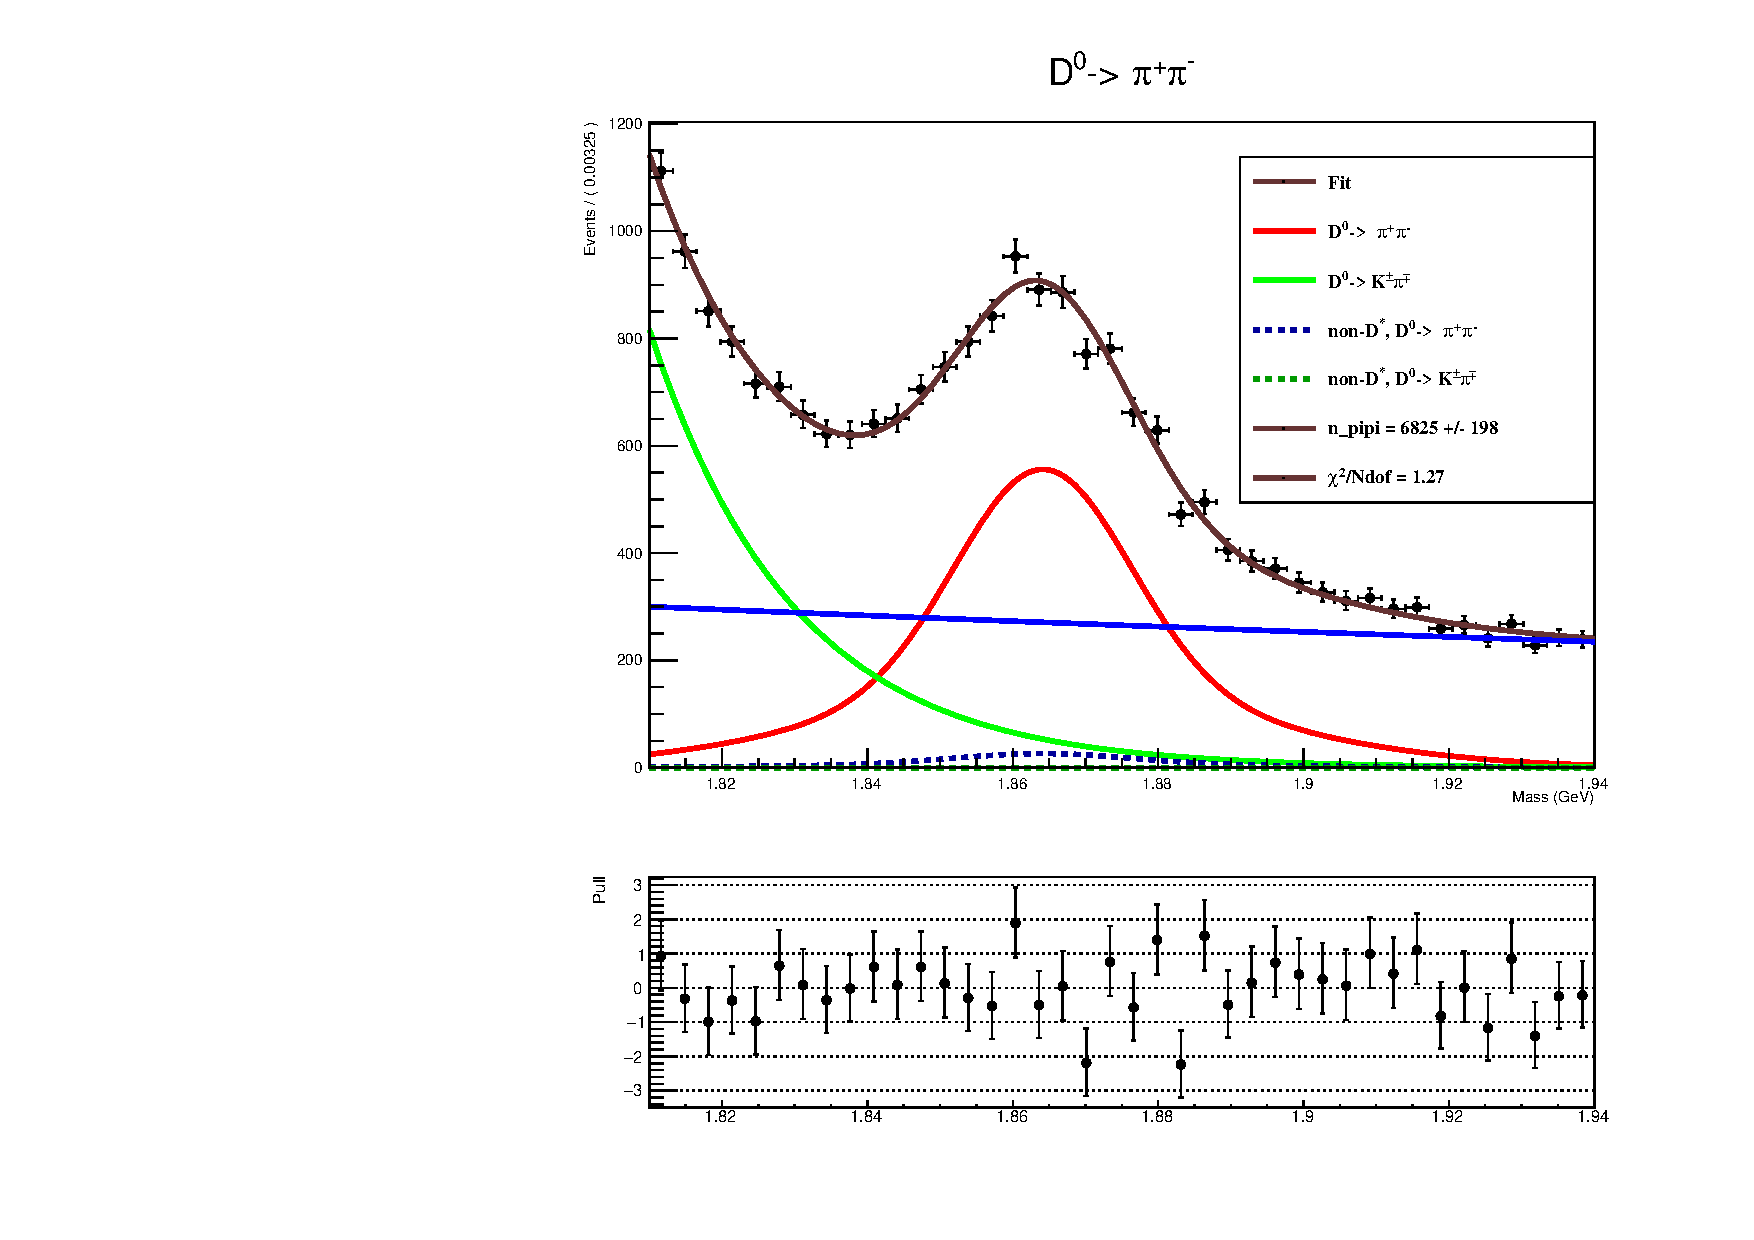
\includegraphics[width=0.45\textwidth]{figures/chapter4/normalization_fit/m_pipiDimuon_afterMvaCut.pdf}
      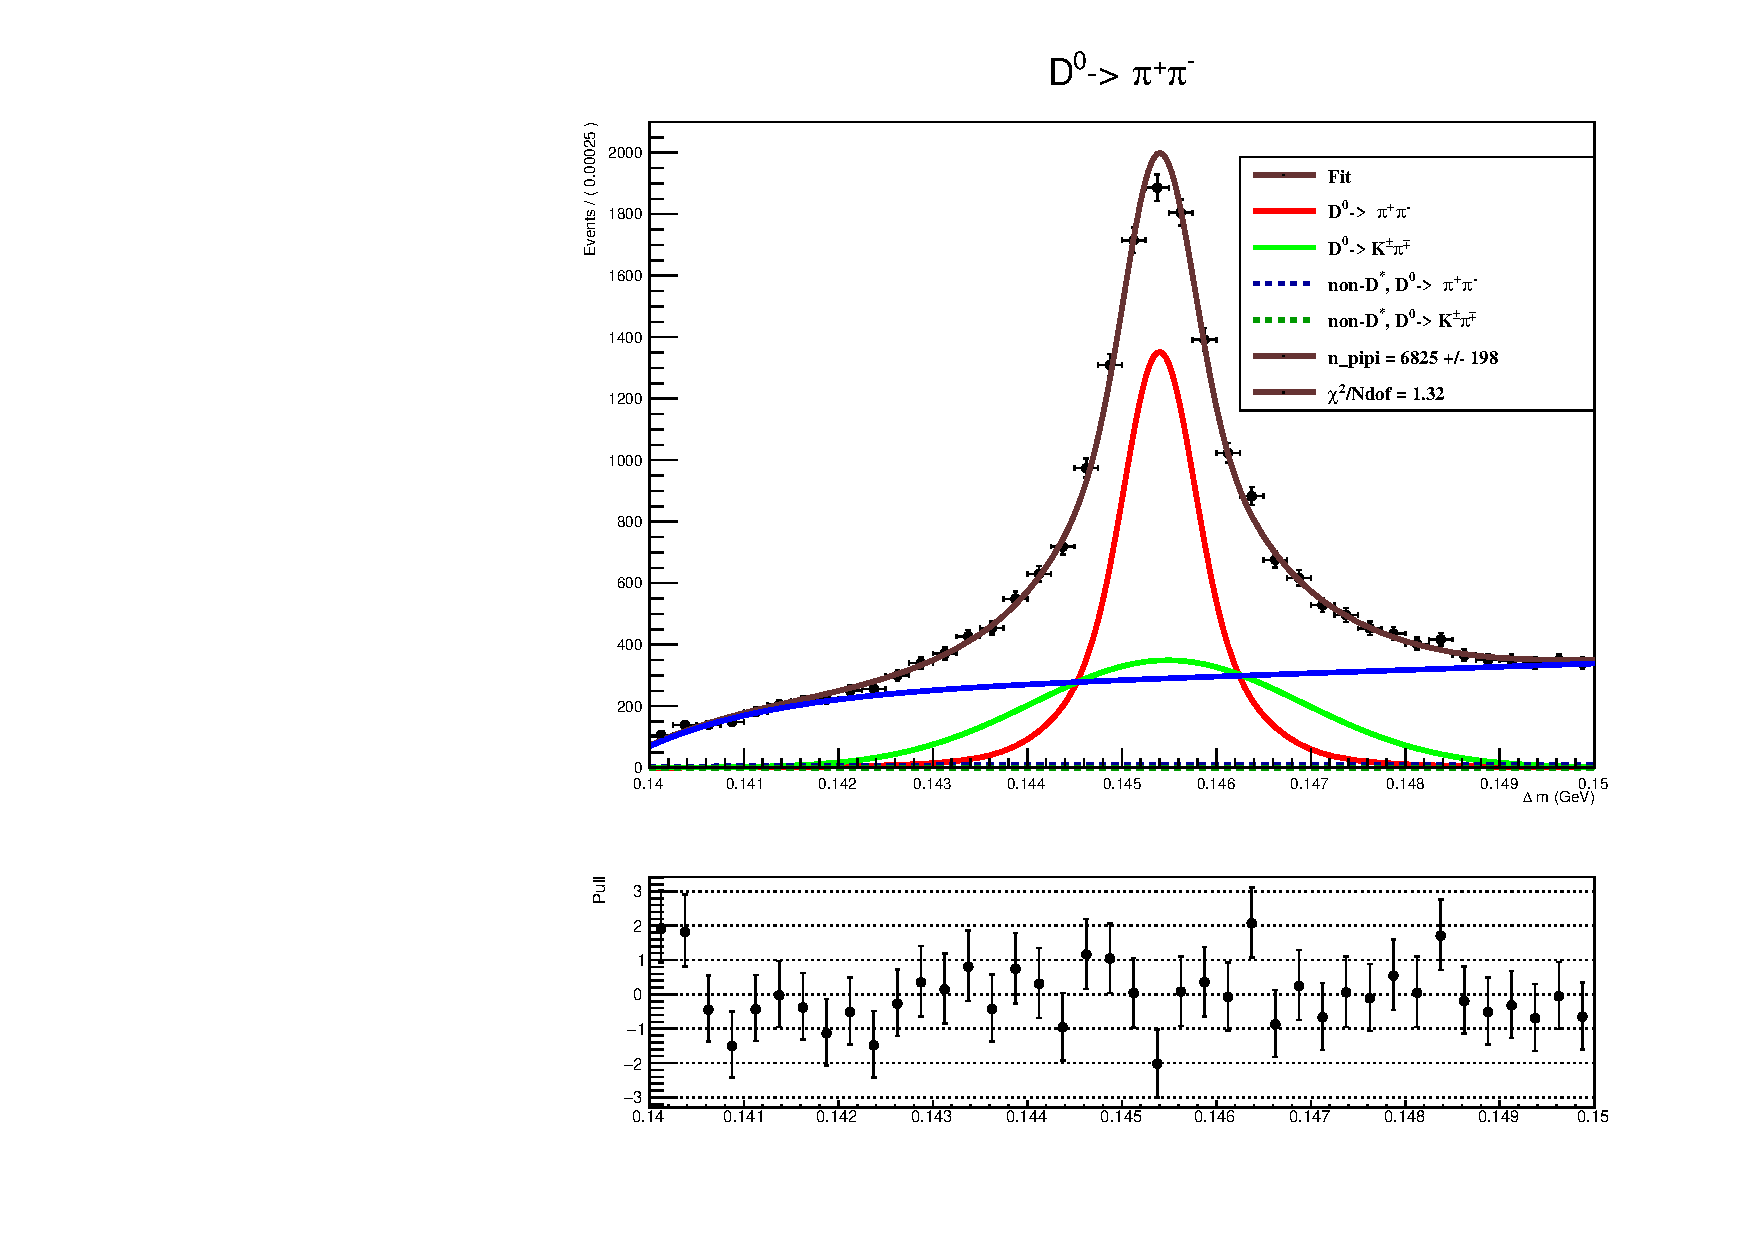
\includegraphics[width=0.45\textwidth]{figures/chapter4/normalization_fit/dm_pipiDimuon_afterMvaCut.pdf}\\
    \end{center}
    \caption{
        The full $D^0 \to \pi^+ \pi^-$ model fit on \texttt{HLT\_ZeroBias} data, with $m(D^0)$ displayed left and $\Delta m$ displayed right.
    }
    \label{fig:d0pipi_uml_fit}
\end{figure}

\begin{figure}[htp]
    \begin{center}
      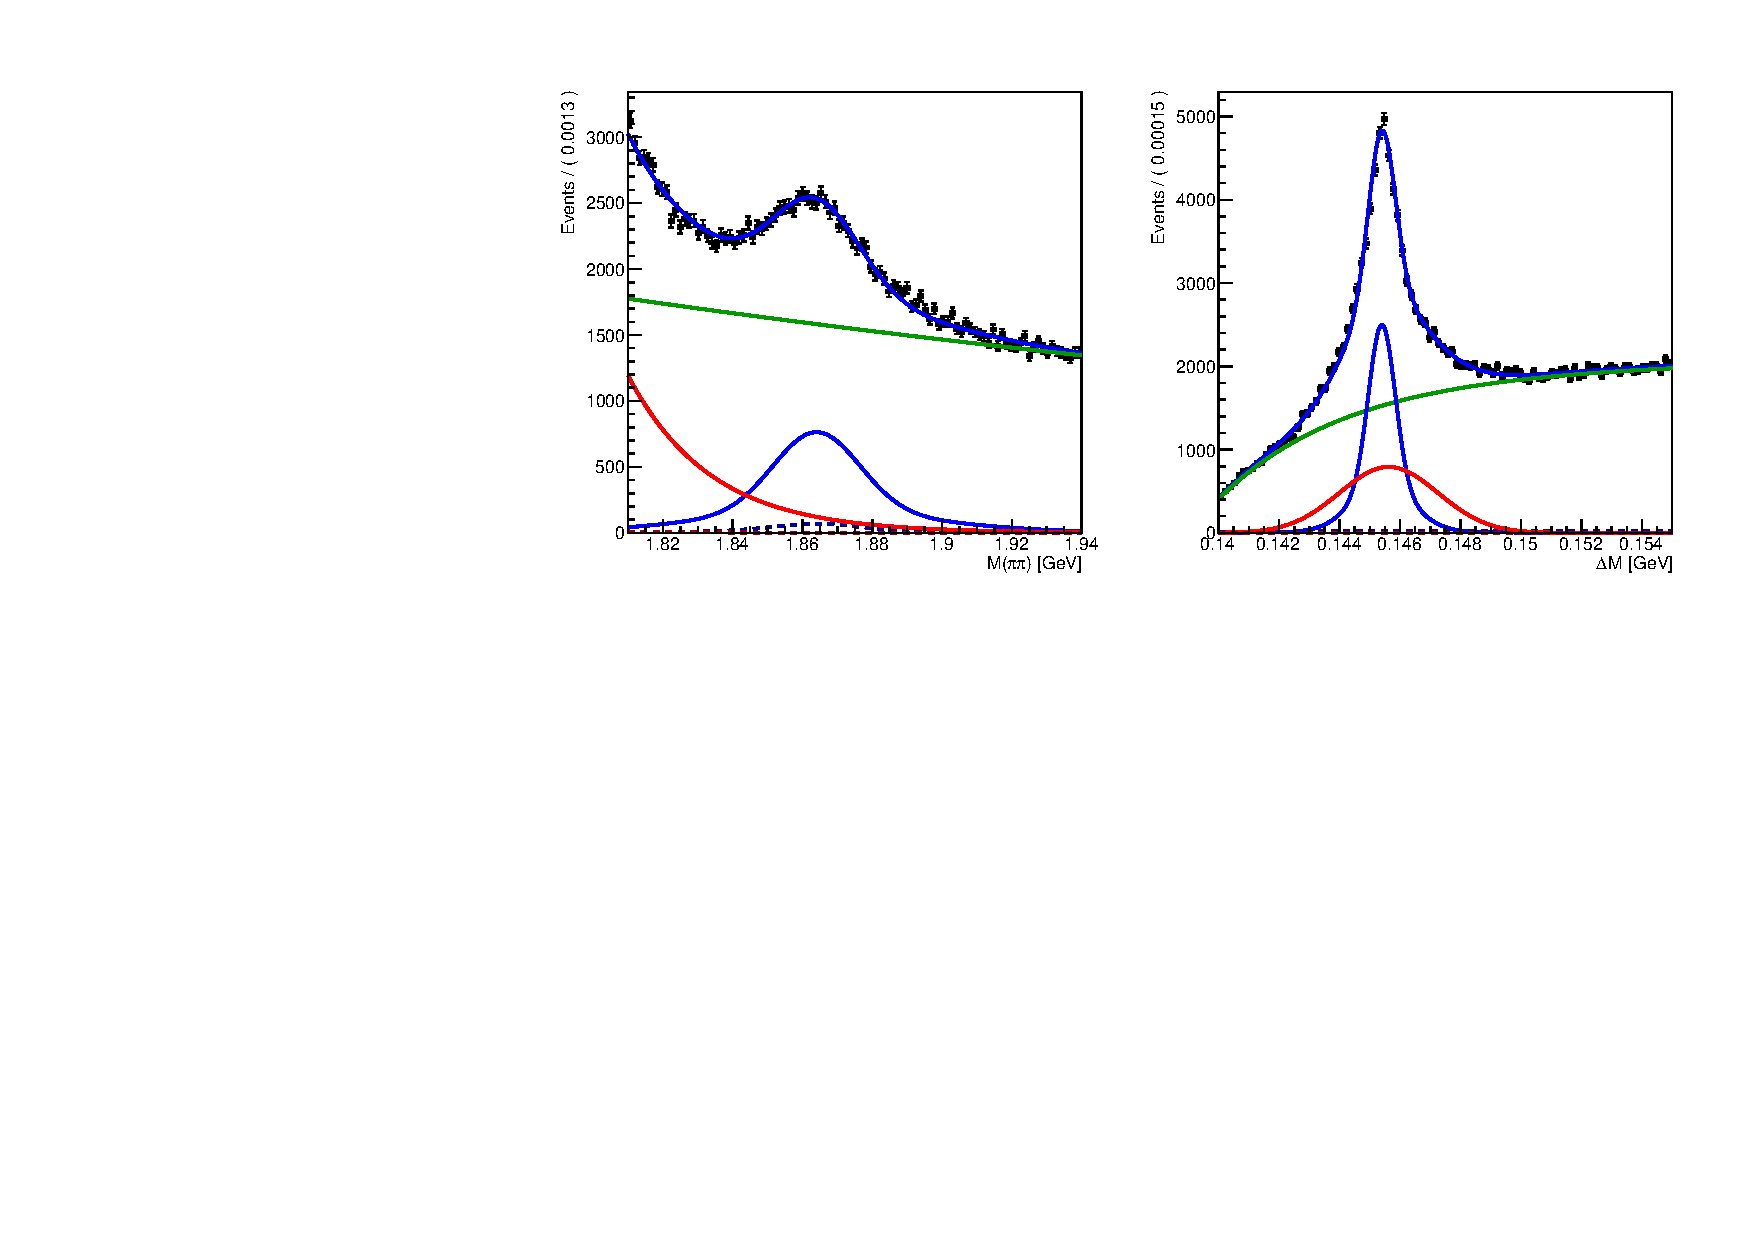
\includegraphics[width=0.9\textwidth]{figures/chapter4/normalization_fit/dpipi_fit.pdf}
    \end{center}
    \caption{
      The full $D^0 \to \pi^+ \pi^-$ model fit on \texttt{HLT\_DoubleMu4\_3\_LowMass} data, with $m(D^0)$ displayed left and $\Delta m$ displayed right. The green line follows the combinatorial model, the blue line follows the signal model, the red line follows the $D^{*\pm} \to D^0\pi^\pm, D^0 \to K^\pm \pi^\mp$ background model, the red dashed line following the non-$D^{*\pm} \to D^0\pi^\pm, D^0 \to K^\pm \pi^\mp$ background model, and the blue dashed line follows the non-$D^{*\pm} \to D^0\pi^\pm, D^0 \to \pi^+ \pi^-$ background model.
    }
    \label{fig:d0pipi_uml_fit_dimuon}
\end{figure}


\begin{table}[h!]
    \centering
    \begin{tabular}{@{}lrr@{}}
    \toprule
    \toprule
    \textbf{\texttt{HLT\_DoubleMu4\_3\_LowMass} data}& Fitted count & Fitted error  \\
    \midrule
    $D^*, D^0 \to \pi\pi$ Yield        & 23787 & $\pm$509 \\
    $D^*, D^0 \to K\pi$ Yield          & 21558  & $\pm$749 \\
    Combinatorial Yield               & 155088 & $\pm$1722 \\
    non--$D^*$, $D^0 \to \pi\pi$ Yield & 2140   & $\pm$685 \\
    non--$D^*$, $D^0 \to K\pi$ Yield   & 181     & $\pm$1410 \\
    \bottomrule
    \toprule
    \textbf{\texttt{HLT\_ZeroBias} data} & Fitted count & Fitted error \\
    \midrule
    $D^*, D^0 \to \pi\pi$ Yield        & 195 & $\pm$17 \\
    $D^*, D^0 \to K\pi$ Yield          & 74  & $\pm$21 \\
    Combinatorial Yield               & 140 & $\pm$20 \\
    non--$D^*$, $D^0 \to \pi\pi$ Yield & 0   & $\pm$11 \\
    non--$D^*$, $D^0 \to K\pi$ Yield   & 0     & $\pm$0 \\
    \bottomrule
    \bottomrule
    \end{tabular}
    \caption{Fitted yields and associated uncertainties for the normalization UML fit.}
    \label{tab:d0pipi_uml_fit_results}
    \end{table}

\subsection{Signal Channel Fit}

The goal of the signal channel is to extract $N_{D^0 \to \mu^+ \mu^-}$. This is done using the \texttt{HLT\_DoubleMu4\_3\_LowMass} trigger dataset, as is described in section \ref{subsec:backgrounds}. As with the normalization channel, the largest difficult of this UML fit is the lack of signal events due to the small branching fraction of the $D^0$ meson. Similarly to the normalization channel, the signal channel uses MC samples to inform the shapes for data, applying corrections when needed. Additionally, the results of the normalization channel are used to fix the background yields. These techniques are described in the remaineder of the section.

It is worth mentioning that much of the machinery needed for this fit has been developed in section \ref{subsec:normalization_channel_fit} and is therefore not repeated here. Namely, this section focuses on the differences in the signal channel that require special attention.

\subsubsection{Signal Model}

The signal model for the normalization channel describes the $\delta M$ and $m(D^0)$ of the $D^{*\pm}\to D^0 \pi^\pm, D^0 \to \pi^+ \pi^-$ decay. The same procedure for determining the normalization channel signal model is used in determining this signal model, with the mean and width corrections derived from the normalization channel.

The signal model fit to MC can be seen in figure \ref{fig:d0mumu_uml_fit}.

\begin{figure}[htp]
    \begin{center}
      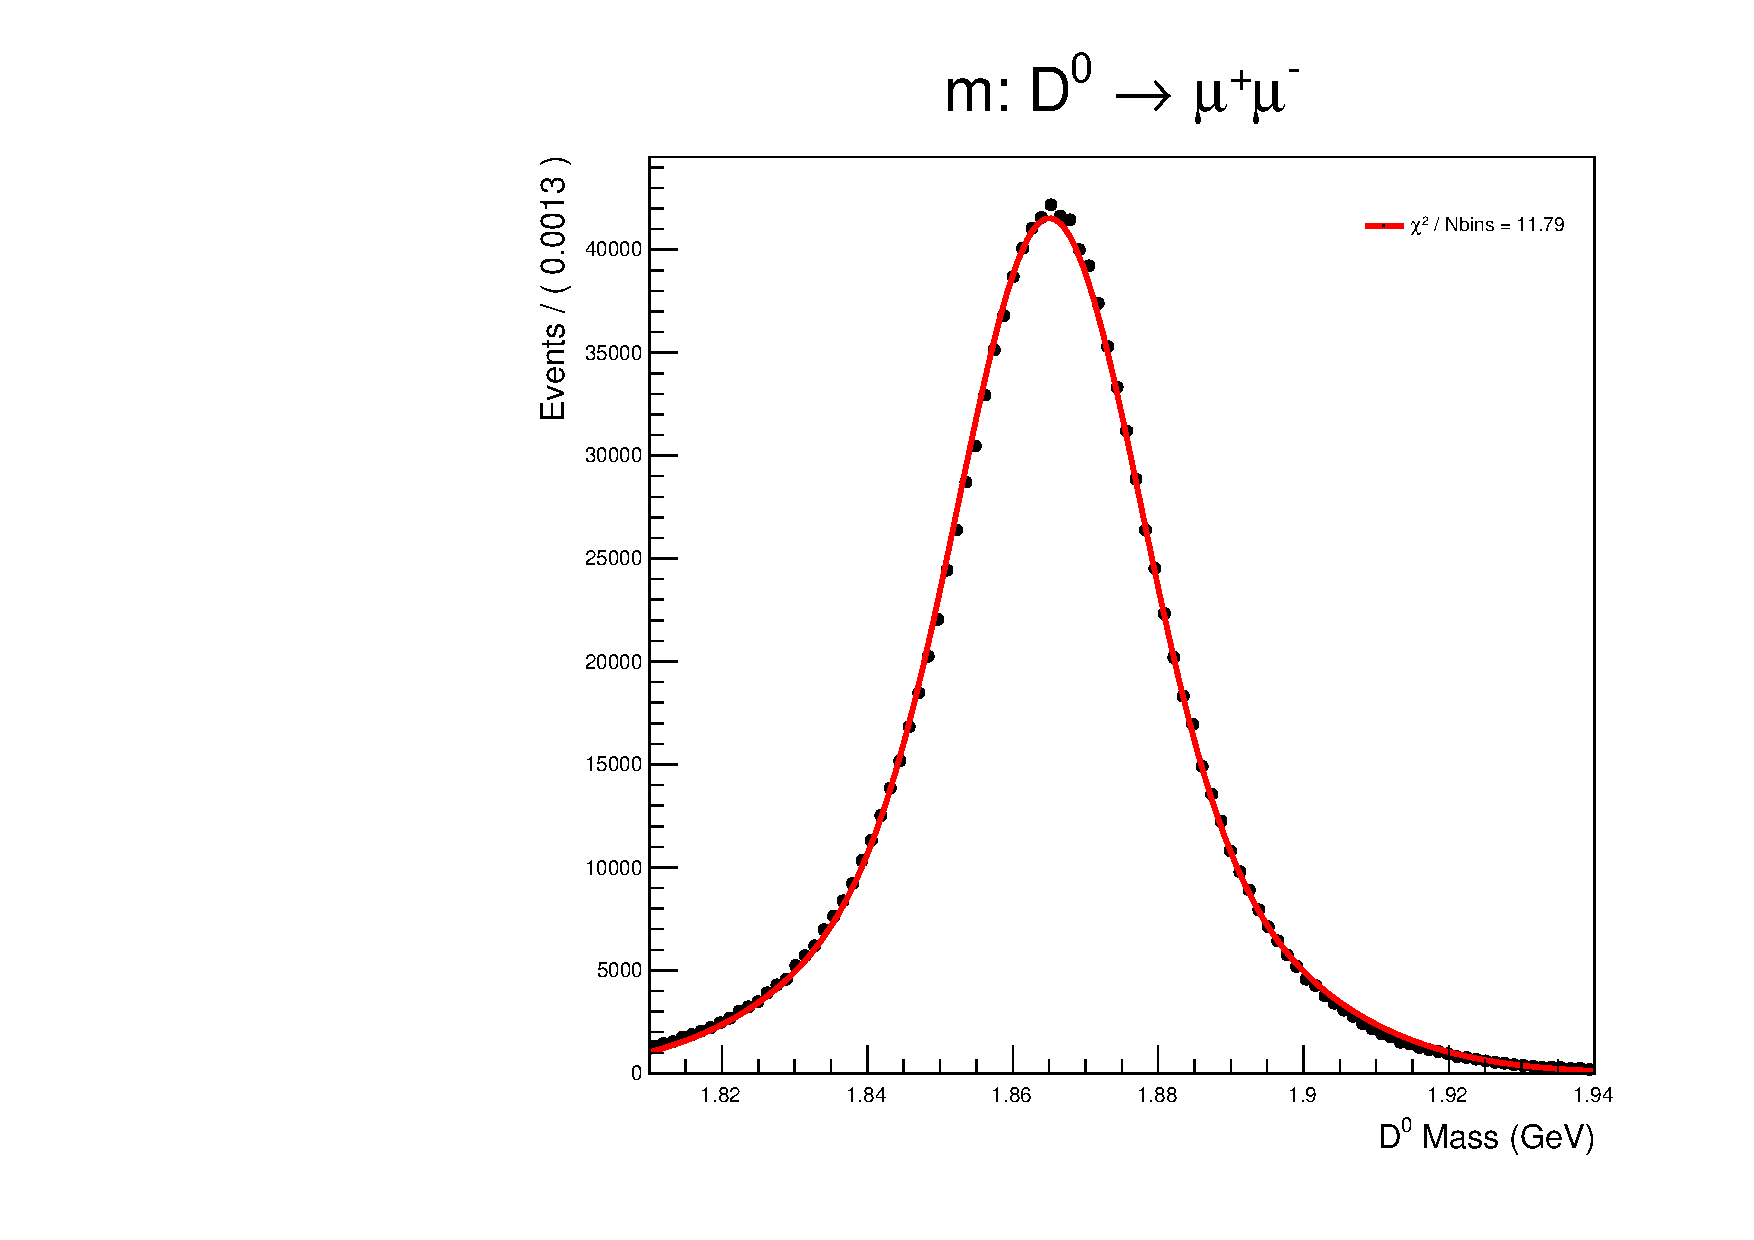
\includegraphics[width=0.45\textwidth]{figures/chapter4/signal_fit/d0mm_2022_2023_0_m.pdf}
      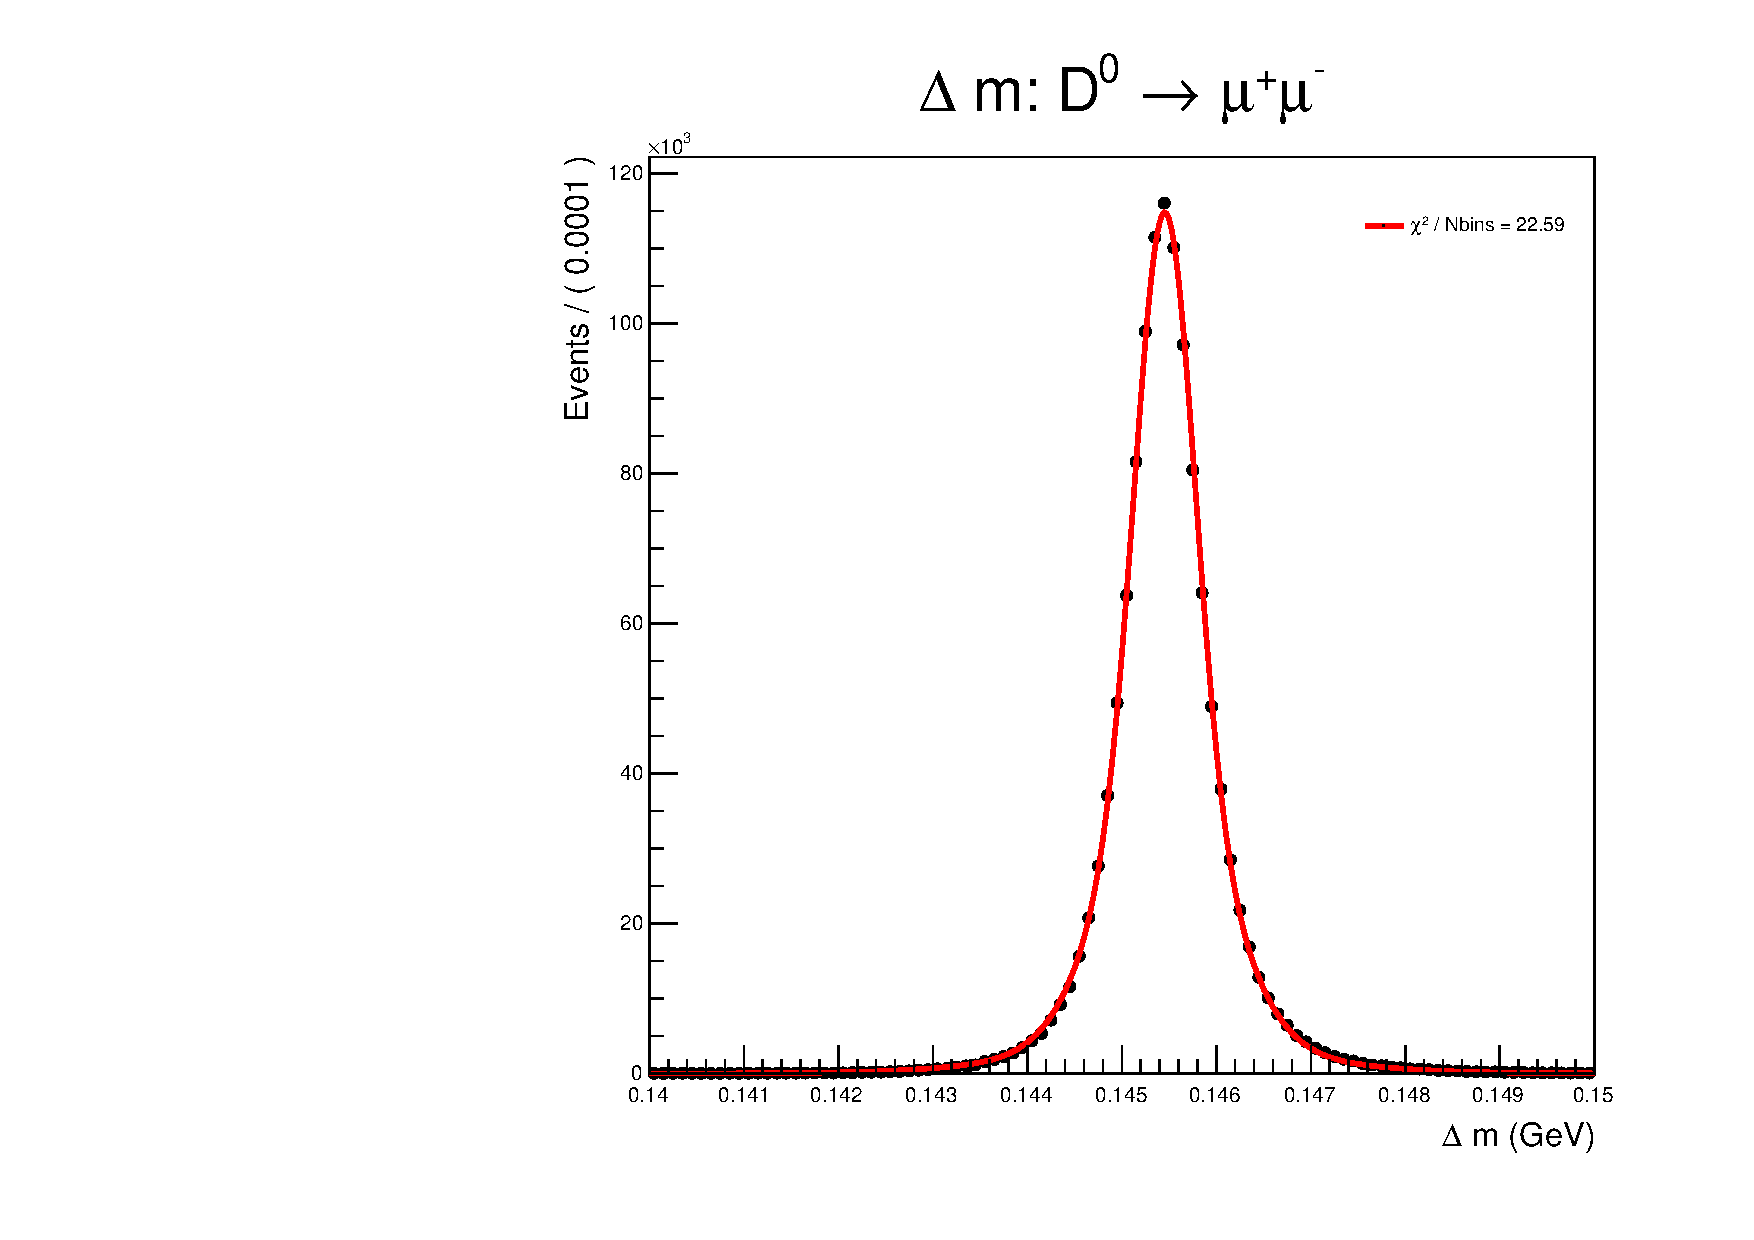
\includegraphics[width=0.45\textwidth]{figures/chapter4/signal_fit/d0mm_2022_2023_0_dm.pdf}\\
    \end{center}
    \caption{
      The signal model fit on MC samples, with $m(D^0)$ displayed left and $\Delta m$ displayed right.
    }
    \label{fig:d0mumu_uml_fit}
\end{figure}

\subsubsection{Background Model}

As is evident from section \ref{subsec:backgrounds}, there are 2 $D^{*\pm} \to D^0 \pi^\pm$ peaking backgrounds and a combinatorial background to consider in the normalization channel. Note that the non-$D^{*\pm} \to D^0 \pi^\pm$ backgrounds which were discussed extensively in the normalization channel are not relevant here due to the large uncertainty of the combinatorial background compared to the expected yield from these backgrounds. Therefore, any non-$D^{*\pm} \to D^0 \pi^\pm$ backgrounds are considered combinatorial and considered in the combinatorial model.

The two peaking backgrounds are $D^{*\pm} \to D^0 \pi^\pm$ processes where the $D^0$ decays via either $D^0 \to \pi^+ \pi^- \to \mu^+ \nu_\mu \mu^- \bar{\nu}_\mu$ (hadronic mode) or via $D^0 \to \to \pi^- \mu^+ \nu_\mu$ (semileptonic mode). Both of these models are developed using the same process as the signal mode. Namely, the models are built out of sums of Gaussian distributions\footnote{Just like in the signal, two Gaussian distributions sharing a common mean are used for $m(D^0)$ and three Gaussian distributions sharing a common mean are used for $\Delta m$}, their shape is determined by fitting to MC samples, and their means and widths are corrected for using the correction derived in the normalization channel fit. 

In the normalization channel, the yields of these models were left floating. In this channel, there are so few events that allowing for this would destabilize the fit. However, we have already calculated $N_{D^0 \to \pi^+ \pi^-} = 195 \pm 17$ in section \ref{subsec:normalization_channel_fit} and the branching fractions of $\mathcal{B}(D^0 \to \pi^+ \pi^-) = (1.454 \pm 0.024) \times 10^{-3}$ and $\mathcal{B}(D^0 \to \pi^-\mu^+ \nu_\mu) = (2.67 \pm 0.12) \times 10^{-3}$ are well known \cite{ref:pdg2024}. Lastly, in section TODO: add fake rate section, we calculate the fake rate, $f_{\pi \to \mu}$, or the rate at which pions decay to muons in the detector, which occurs once in the semi-leptonic mode and twice in the hadronic mode.

Using these qualities, as well as efficiency and MC corrections, we can write
\begin{equation}
\begin{split}
    \frac{N_{D^0 \to \pi^+ \pi^- \to \mu^+ \nu_\mu \mu^- \bar{\nu}_\mu}}{N_{D^0 \to \pi^+ \pi^-}} &= \left(f_{\pi \to \mu}\right)^2 \times \frac{\epsilon_{D^*, D^0\to\pi\pi\to\mu\mu}}{\epsilon_{D^*, D^0\to\pi\pi}} \times S_{ZB} \times \text{MVA}_D \times T_{\text{corr}} \\
    \frac{N_{D^0 \to \pi^- \mu^ \nu_\mu}}{N_{D^0 \to \pi^+ \pi^-}} &=\frac{\mathcal{B}_{D^0 \to \pi^- \mu^ \nu_\mu}}{\mathcal{B}_{D^0 \to \pi^+ \pi^-}} \times \left(f_{\pi \to \mu}\right) \times \frac{\epsilon_{D^*, D^0\to\pi\mu\nu}}{\epsilon_{D^*, D^0\to\pi\pi}} \times S_{ZB} \times \text{MVA}_D \times T_{\text{corr}}
    \label{eq:peaking_background_yield_calculation}
\end{split}
\end{equation}
where $S_{ZB}$ is the trigger prescaling factor discussed in section $\ref{subsec:data_samples}$, $\epsilon$ is the efficiency discussed in section \ref{subsec:baseline_selection}, $\text{MVA}_D$ is the MVA correction discussed in section $\ref{subsec:mva}$, and $T_{\text{corr}}$ are the trigger corrections discussed in section TODO: add trigger correction section. The convergence of the two fits in MC is shown in figure \ref{fig:d0pimunu_uml_fit} and figure \ref{fig:d0munumunu_uml_fit}

\begin{figure}[htp]
    \begin{center}
      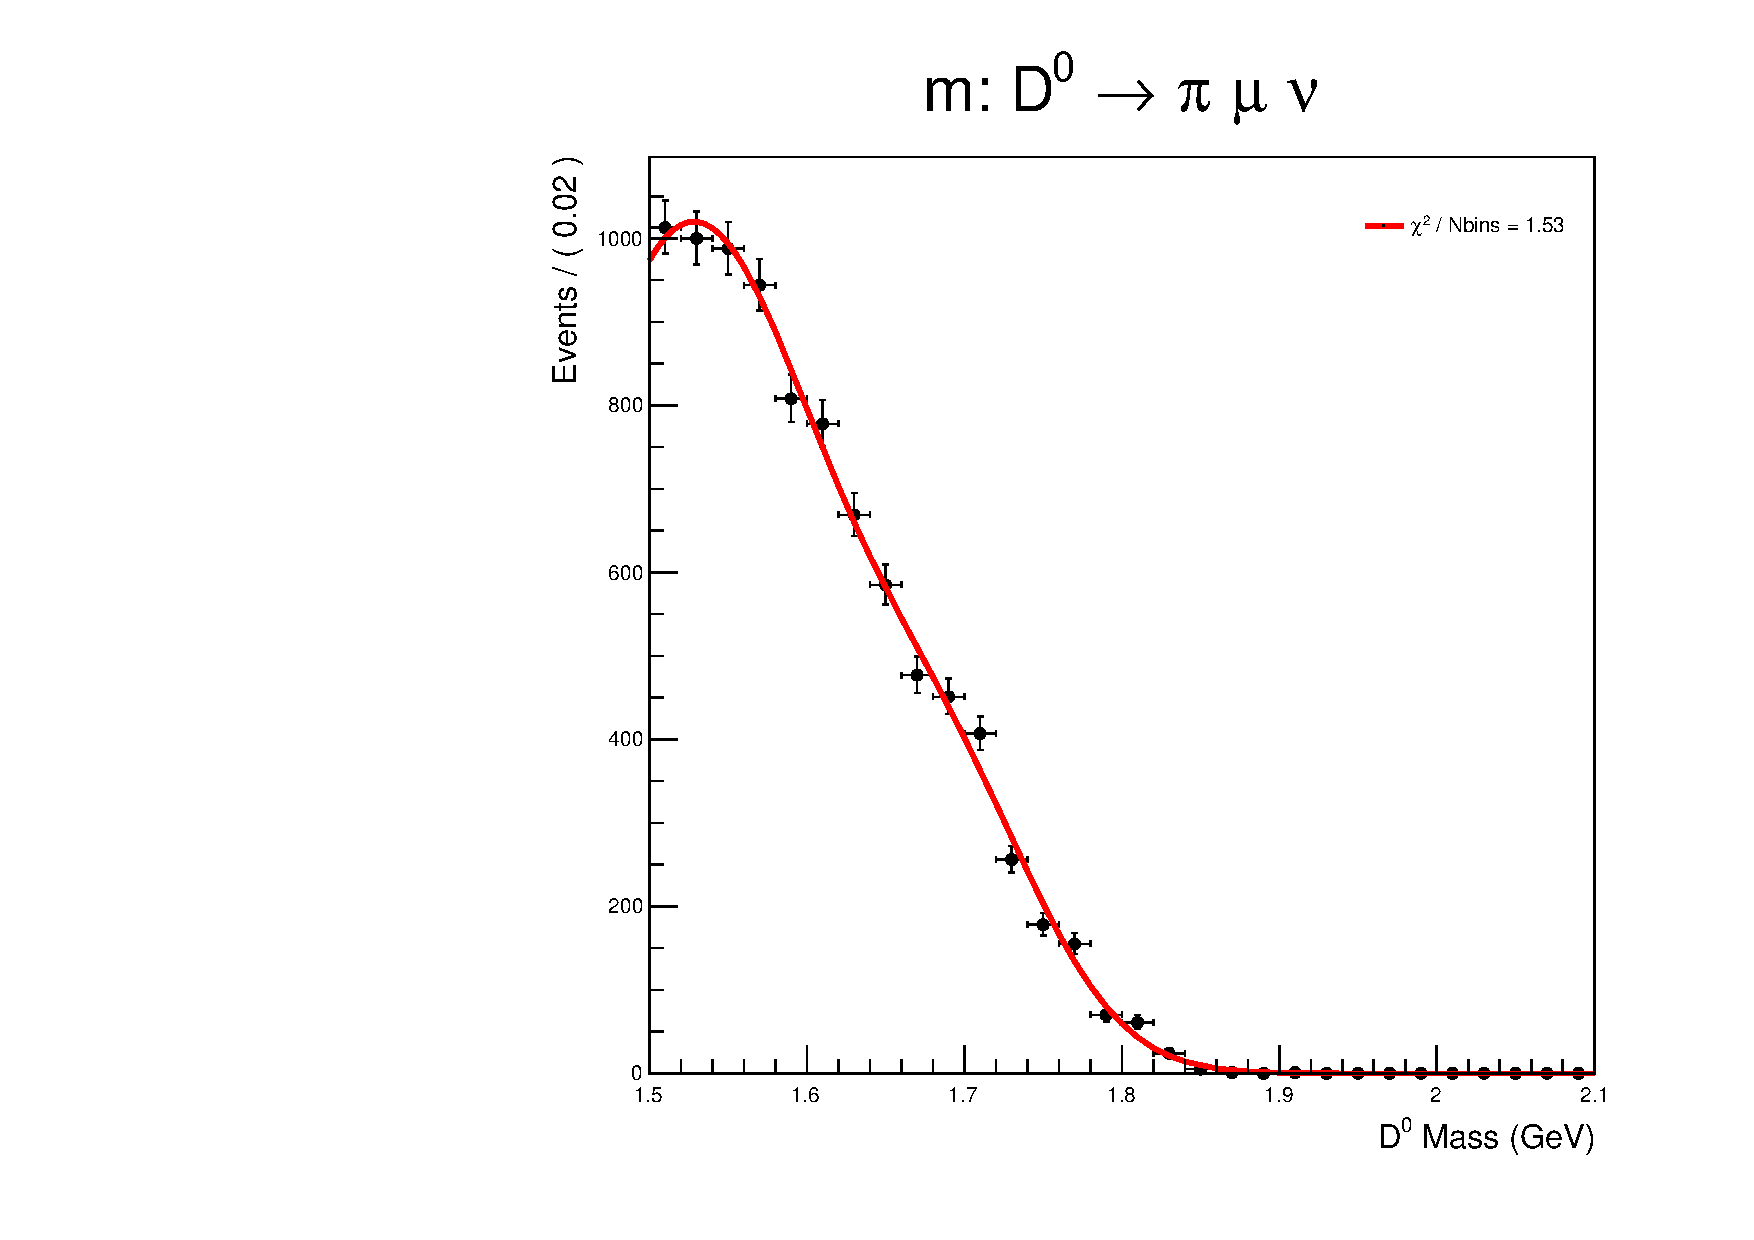
\includegraphics[width=0.45\textwidth]{figures/chapter4/signal_fit/d0pimunu_2022_2023_0_m.pdf}
      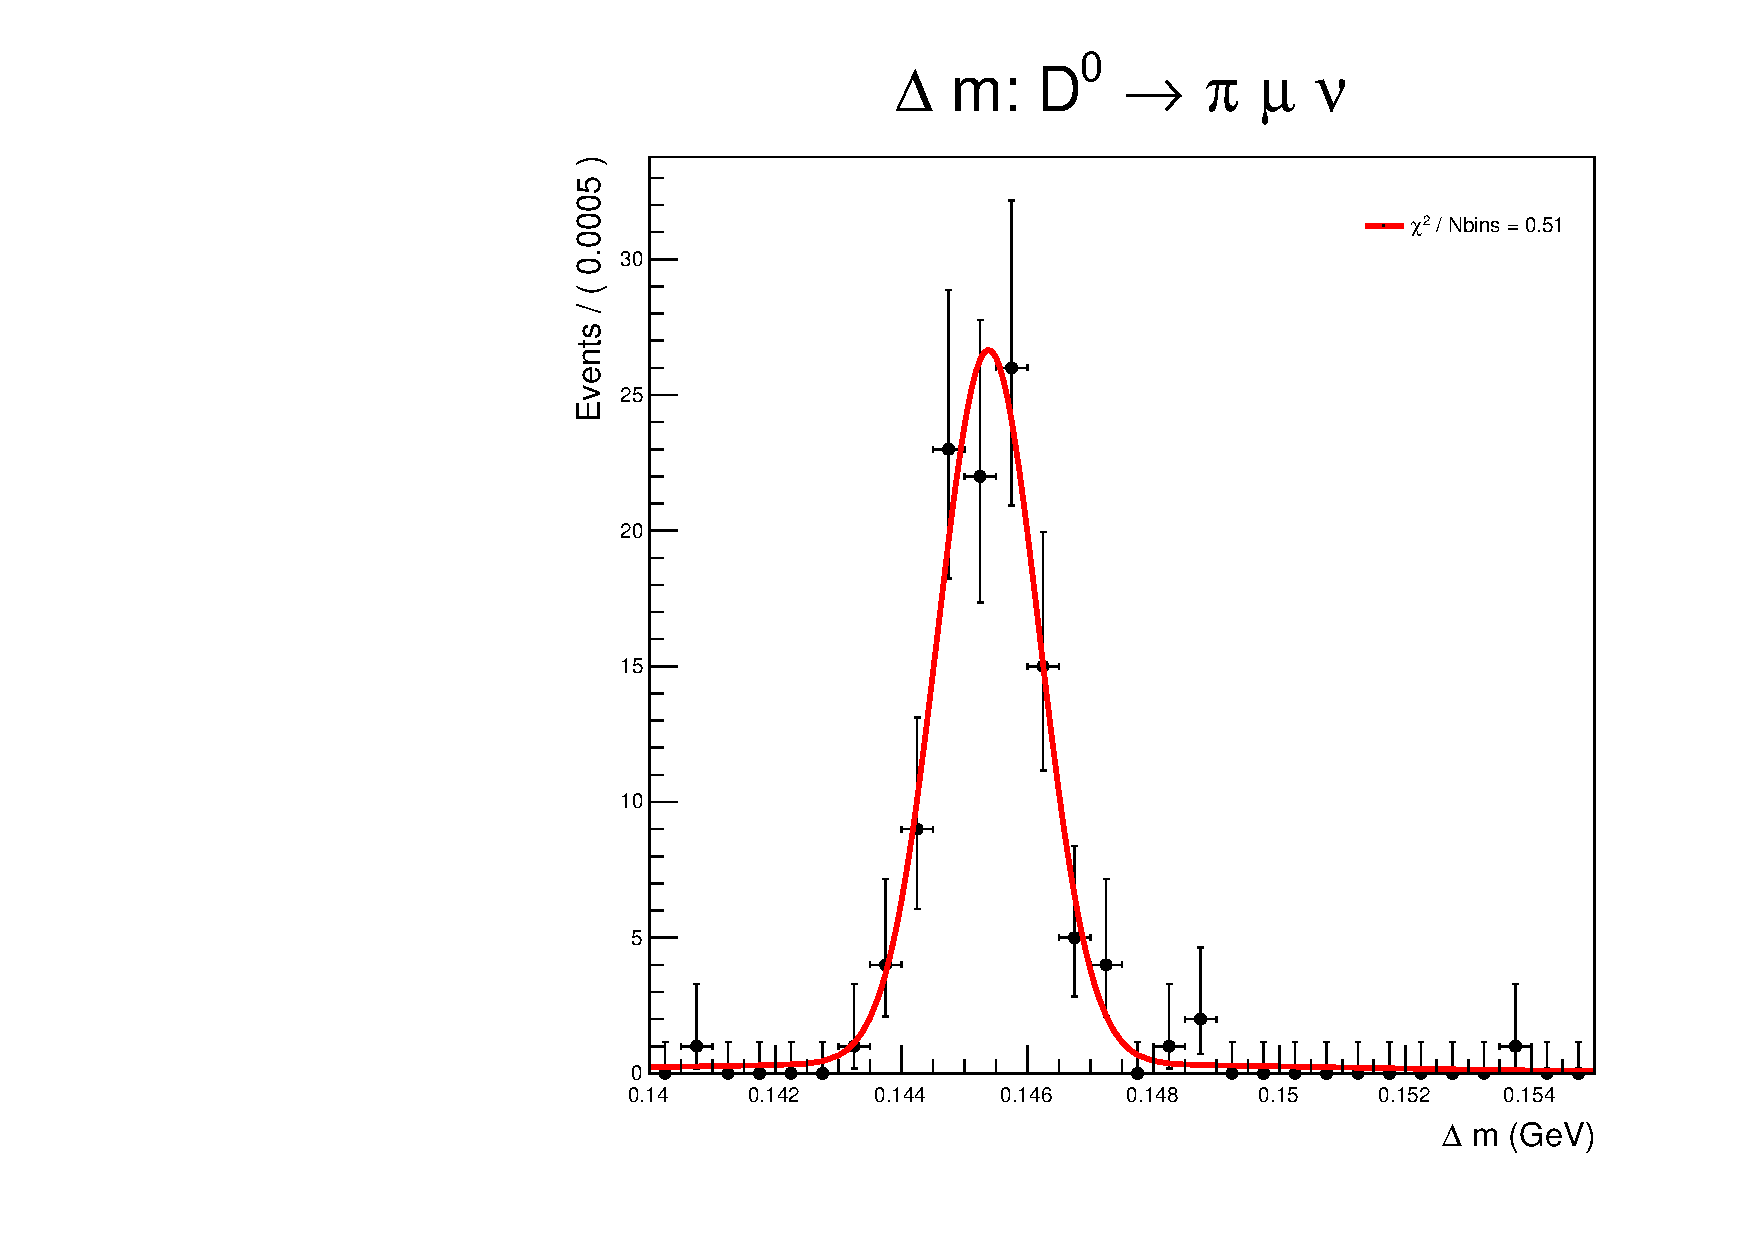
\includegraphics[width=0.45\textwidth]{figures/chapter4/signal_fit/d0pimunu_2022_2023_0_dm.pdf}\\
    \end{center}
    \caption{
      The $D^{*\pm} \to D^0\pi^\pm, D^0 \to \to \pi^- \mu^+ \nu_\mu$ model fit on MC samples, with $m(D^0)$ displayed left and $\Delta m$ displayed right.
    }
    \label{fig:d0pimunu_uml_fit}
\end{figure}

\begin{figure}[htp]
    \begin{center}
      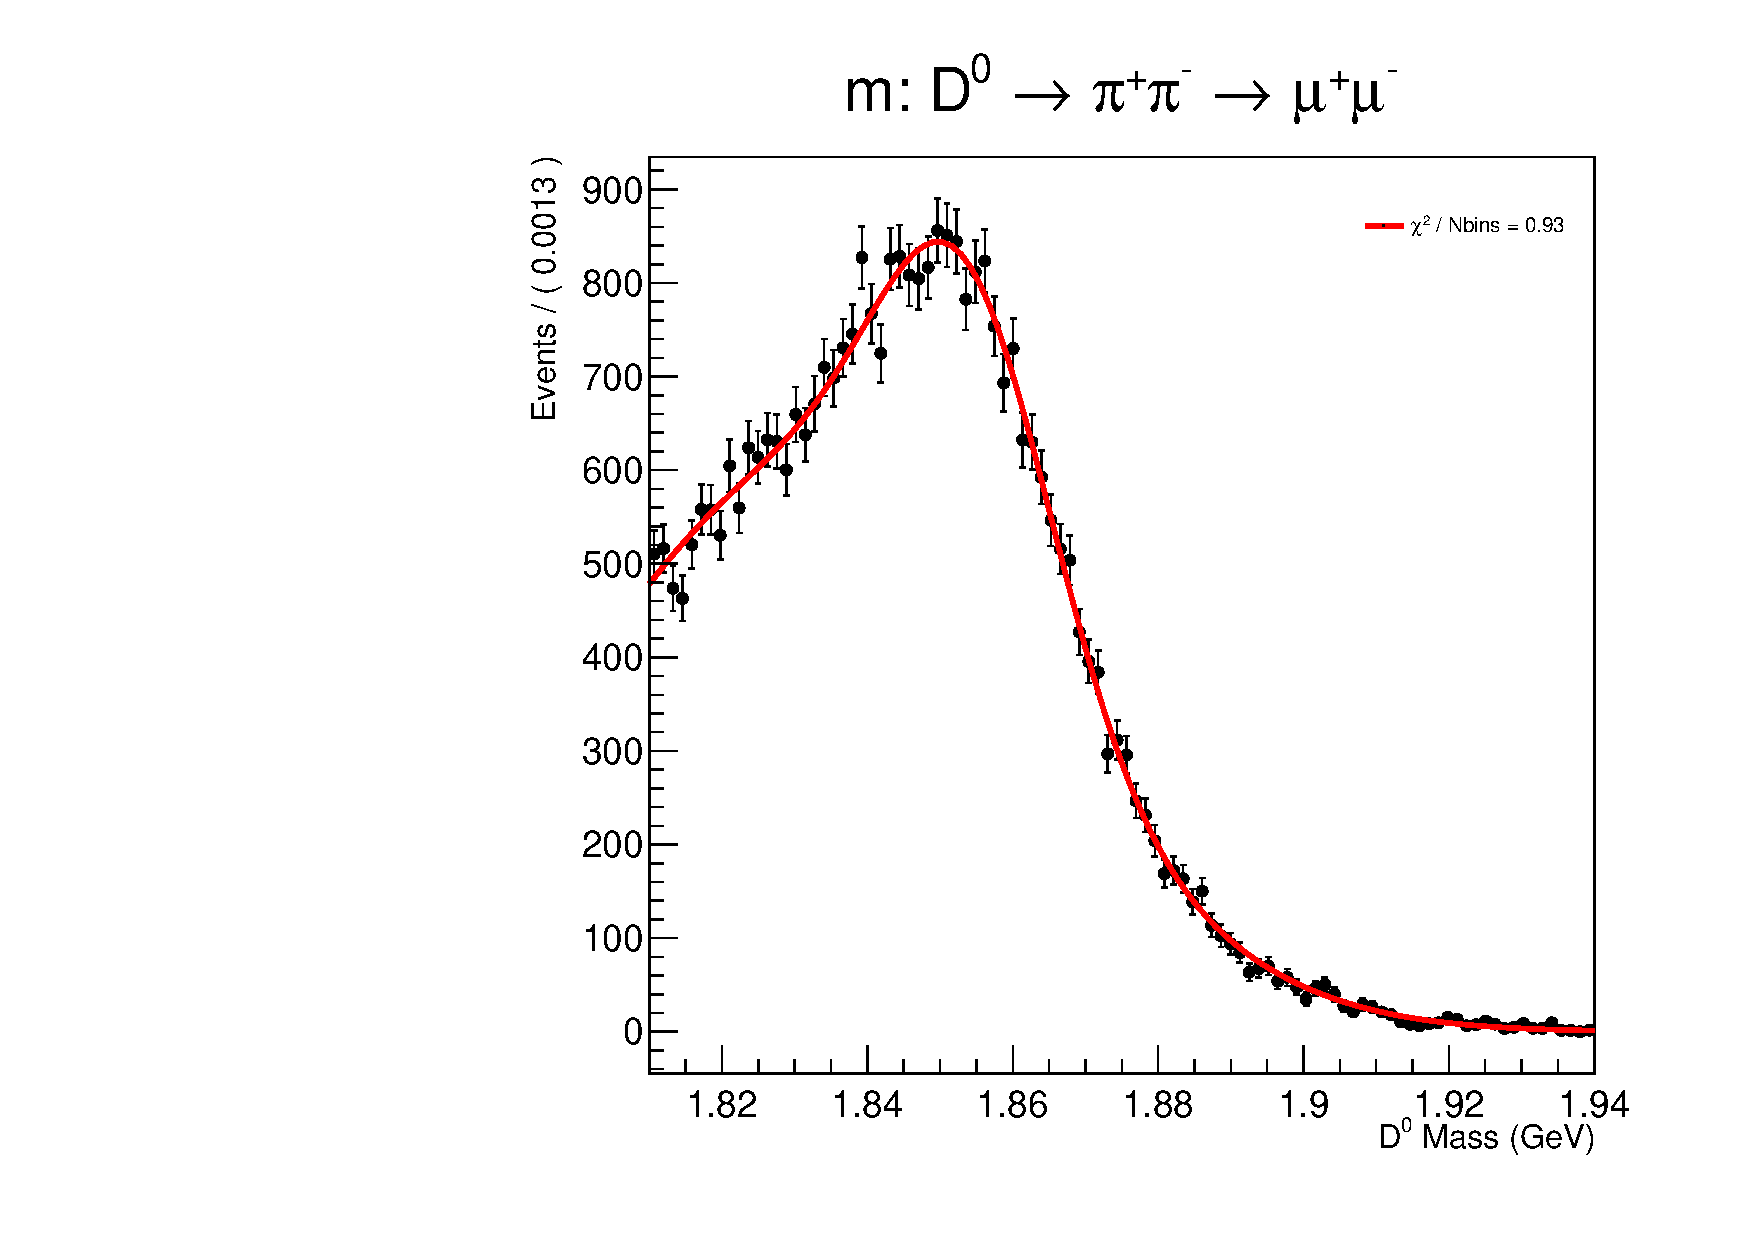
\includegraphics[width=0.45\textwidth]{figures/chapter4/signal_fit/d0pipimm_2022_2023_0_m.pdf}
      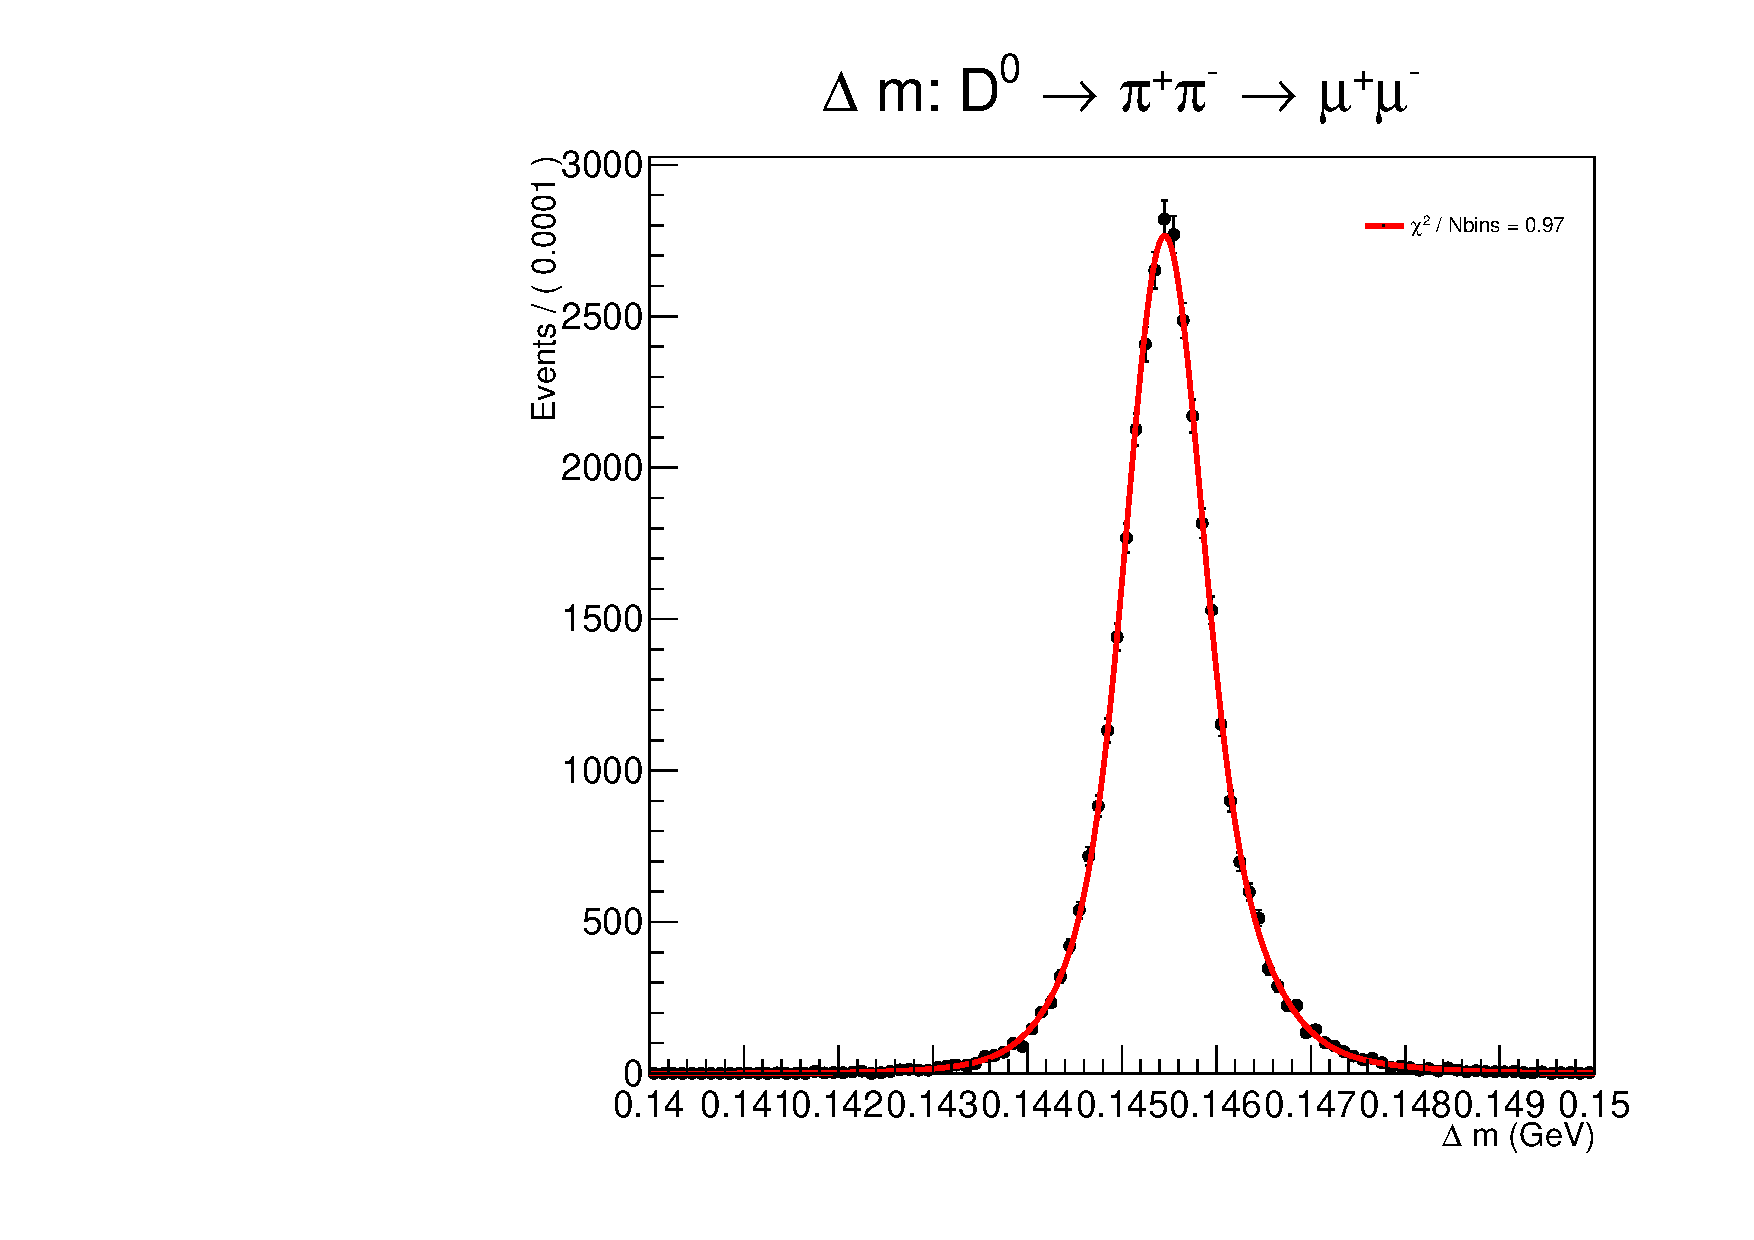
\includegraphics[width=0.45\textwidth]{figures/chapter4/signal_fit/d0pipimm_2022_2023_0_dm.pdf}\\
    \end{center}
    \caption{
      The $D^{*\pm} \to D^0\pi^\pm, D^0 \to \pi^+ \pi^- \to \mu^+ \nu_\mu \mu^- \bar{\nu}_\mu$ model fit on MC samples, with $m(D^0)$ displayed left and $\Delta m$ displayed right.
    }
    \label{fig:d0munumunu_uml_fit}
\end{figure}


The process for determining the combinatorial model is kept the same as for the normalization channel. The only difference is that due to the added complexity of the backgrounds, the $m(D^0)$ pdf function is a combination of a Bernstein polynomial, power law, and exponential function, instead of just an exponential function as was used in the normalization channel. Similar to the normalization channel, the shape and yield is determined using data side-bands, leaving no combinatorial variables left to fit in the main data region.

\subsubsection{Fit Results}

The final model used for the fit is a sum of signal model and all the background models. One important note is to emphasize that the signal shape and peaking background shape are entirely deriving from MC, the peaking background yeild is determined from equation \ref{eq:peaking_background_yield_calculation}, and combinatorial background shape and yield are determined by the data side-bands. Therefore, the only parameter of this fit is the actual parameter of interest, namely the $N_{D^0 \to \pi^+ \pi^-}$ events. 

The results of this fit are only seen after unblinding the data in as discussed in section \ref{sec:analysis_overview}. Therefore, the results are presented in section TODO: add section of this thesis. 